% Options for packages loaded elsewhere
% Options for packages loaded elsewhere
\PassOptionsToPackage{unicode}{hyperref}
\PassOptionsToPackage{hyphens}{url}
\PassOptionsToPackage{dvipsnames,svgnames,x11names}{xcolor}
%
\documentclass[
  chinese,
  letterpaper,
  DIV=11,
  numbers=noendperiod]{scrartcl}
\usepackage{xcolor}
\usepackage{amsmath,amssymb}
\setcounter{secnumdepth}{-\maxdimen} % remove section numbering
\usepackage{iftex}
\ifPDFTeX
  \usepackage[T1]{fontenc}
  \usepackage[utf8]{inputenc}
  \usepackage{textcomp} % provide euro and other symbols
\else % if luatex or xetex
  \usepackage{unicode-math} % this also loads fontspec
  \defaultfontfeatures{Scale=MatchLowercase}
  \defaultfontfeatures[\rmfamily]{Ligatures=TeX,Scale=1}
\fi
\usepackage{lmodern}
\ifPDFTeX\else
  % xetex/luatex font selection
\fi
% Use upquote if available, for straight quotes in verbatim environments
\IfFileExists{upquote.sty}{\usepackage{upquote}}{}
\IfFileExists{microtype.sty}{% use microtype if available
  \usepackage[]{microtype}
  \UseMicrotypeSet[protrusion]{basicmath} % disable protrusion for tt fonts
}{}
\makeatletter
\@ifundefined{KOMAClassName}{% if non-KOMA class
  \IfFileExists{parskip.sty}{%
    \usepackage{parskip}
  }{% else
    \setlength{\parindent}{0pt}
    \setlength{\parskip}{6pt plus 2pt minus 1pt}}
}{% if KOMA class
  \KOMAoptions{parskip=half}}
\makeatother
% Make \paragraph and \subparagraph free-standing
\makeatletter
\ifx\paragraph\undefined\else
  \let\oldparagraph\paragraph
  \renewcommand{\paragraph}{
    \@ifstar
      \xxxParagraphStar
      \xxxParagraphNoStar
  }
  \newcommand{\xxxParagraphStar}[1]{\oldparagraph*{#1}\mbox{}}
  \newcommand{\xxxParagraphNoStar}[1]{\oldparagraph{#1}\mbox{}}
\fi
\ifx\subparagraph\undefined\else
  \let\oldsubparagraph\subparagraph
  \renewcommand{\subparagraph}{
    \@ifstar
      \xxxSubParagraphStar
      \xxxSubParagraphNoStar
  }
  \newcommand{\xxxSubParagraphStar}[1]{\oldsubparagraph*{#1}\mbox{}}
  \newcommand{\xxxSubParagraphNoStar}[1]{\oldsubparagraph{#1}\mbox{}}
\fi
\makeatother


\usepackage{longtable,booktabs,array}
\newcounter{none} % for unnumbered tables
\usepackage{calc} % for calculating minipage widths
% Correct order of tables after \paragraph or \subparagraph
\usepackage{etoolbox}
\makeatletter
\patchcmd\longtable{\par}{\if@noskipsec\mbox{}\fi\par}{}{}
\makeatother
% Allow footnotes in longtable head/foot
\IfFileExists{footnotehyper.sty}{\usepackage{footnotehyper}}{\usepackage{footnote}}
\makesavenoteenv{longtable}
\usepackage{graphicx}
\makeatletter
\newsavebox\pandoc@box
\newcommand*\pandocbounded[1]{% scales image to fit in text height/width
  \sbox\pandoc@box{#1}%
  \Gscale@div\@tempa{\textheight}{\dimexpr\ht\pandoc@box+\dp\pandoc@box\relax}%
  \Gscale@div\@tempb{\linewidth}{\wd\pandoc@box}%
  \ifdim\@tempb\p@<\@tempa\p@\let\@tempa\@tempb\fi% select the smaller of both
  \ifdim\@tempa\p@<\p@\scalebox{\@tempa}{\usebox\pandoc@box}%
  \else\usebox{\pandoc@box}%
  \fi%
}
% Set default figure placement to htbp
\def\fps@figure{htbp}
\makeatother



\ifLuaTeX
\usepackage[bidi=basic,shorthands=off,provide=*]{babel}
\else
\usepackage[bidi=default,shorthands=off,provide=*]{babel}
\fi
\ifLuaTeX
  \usepackage{selnolig} % disable illegal ligatures
\fi


\setlength{\emergencystretch}{3em} % prevent overfull lines

\providecommand{\tightlist}{%
  \setlength{\itemsep}{0pt}\setlength{\parskip}{0pt}}



 


\KOMAoption{captions}{tableheading}
\makeatletter
\@ifpackageloaded{caption}{}{\usepackage{caption}}
\AtBeginDocument{%
\ifdefined\contentsname
  \renewcommand*\contentsname{目录}
\else
  \newcommand\contentsname{目录}
\fi
\ifdefined\listfigurename
  \renewcommand*\listfigurename{图索引}
\else
  \newcommand\listfigurename{图索引}
\fi
\ifdefined\listtablename
  \renewcommand*\listtablename{表索引}
\else
  \newcommand\listtablename{表索引}
\fi
\ifdefined\figurename
  \renewcommand*\figurename{图}
\else
  \newcommand\figurename{图}
\fi
\ifdefined\tablename
  \renewcommand*\tablename{表}
\else
  \newcommand\tablename{表}
\fi
}
\@ifpackageloaded{float}{}{\usepackage{float}}
\floatstyle{ruled}
\@ifundefined{c@chapter}{\newfloat{codelisting}{h}{lop}}{\newfloat{codelisting}{h}{lop}[chapter]}
\floatname{codelisting}{列表}
\newcommand*\listoflistings{\listof{codelisting}{列表索引}}
\makeatother
\makeatletter
\makeatother
\makeatletter
\@ifpackageloaded{caption}{}{\usepackage{caption}}
\@ifpackageloaded{subcaption}{}{\usepackage{subcaption}}
\makeatother
\usepackage{bookmark}
\IfFileExists{xurl.sty}{\usepackage{xurl}}{} % add URL line breaks if available
\urlstyle{same}
% fallback for those not using the hyperref driver hyperxmp:
\makeatletter
\@ifundefined{xmpquote}{\newcommand{\xmpquote}[1]{#1}}{}
\makeatother
\hypersetup{
  pdftitle={静岸 · 操作说明书},
  pdflang={zh-CN},
  colorlinks=true,
  linkcolor={blue},
  filecolor={Maroon},
  citecolor={Blue},
  urlcolor={Blue},
  pdfcreator={LaTeX via pandoc}}


\title{静岸 · 操作说明书}
\usepackage{etoolbox}
\makeatletter
\providecommand{\subtitle}[1]{% add subtitle to \maketitle
  \apptocmd{\@title}{\par {\large #1 \par}}{}{}
}
\makeatother
\subtitle{场景化排尿引导器 / 场景化问卷作答器}
\author{}
\date{Invalid Date}
\begin{document}
\maketitle


QUIET SHORE VR

静岸 · 操作说明书

场景化排尿引导器场景化问卷作答器

v2.1 · 2026-11-14

读者：床边操作的技术员

PICO G2 4K 头显 ＋ 10 英寸 Android 平板

\section{一页速查}\label{ux4e00ux9875ux901fux67e5}

{\def\LTcaptype{none} % do not increment counter
\begin{longtable}[]{@{}
  >{\raggedright\arraybackslash}p{(\linewidth - 2\tabcolsep) * \real{0.5000}}
  >{\raggedright\arraybackslash}p{(\linewidth - 2\tabcolsep) * \real{0.5000}}@{}}
\toprule\noalign{}
\begin{minipage}[b]{\linewidth}\raggedright
要做的事
\end{minipage} & \begin{minipage}[b]{\linewidth}\raggedright
在哪里
\end{minipage} \\
\midrule\noalign{}
\endhead
\bottomrule\noalign{}
\endlastfoot
连接头显 & 首页右侧「头显」窗口 → 搜索头显 → 连接 \\
切换应用 & 顶栏当前应用名；会话中锁定 \\
看当前应用的说明书 & 左侧 \texttt{说明} 页签 \\
开始训练 & 场景化排尿引导器 → 场景页右侧「启动训练」 \\
结束会话 & 会话页底部「结束会话」 \\
断开链接（急停） & 顶栏右侧；立即冻结，5 秒未重连则头显退出场景回首页 \\
作答与归档 & 顶栏切到「场景化问卷作答器」 \\
导出记录 & 场景化问卷作答器 → 归档 → 导出 \\
导出体验 CSV & 场景化排尿引导器 → 体验 → 导出 CSV \\
\end{longtable}
}

\textbf{患者只做一件事：戴上头显后，按一次头显右侧按钮进入画面。}
开始、停止、体位与场景都由平板操作员控制。

\section{1
这套系统怎么用}\label{ux8fd9ux5957ux7cfbux7edfux600eux4e48ux7528}

静岸是一套床边的场景体验。患者躺卧或半躺时，头显呈现近似站立时的视野；画面与声音节奏由床边的技术员掌握。

系统有两个并列的应用面，由顶栏的应用选择器切换：

{\def\LTcaptype{none} % do not increment counter
\begin{longtable}[]{@{}
  >{\raggedright\arraybackslash}p{(\linewidth - 2\tabcolsep) * \real{0.5000}}
  >{\raggedright\arraybackslash}p{(\linewidth - 2\tabcolsep) * \real{0.5000}}@{}}
\toprule\noalign{}
\begin{minipage}[b]{\linewidth}\raggedright
应用
\end{minipage} & \begin{minipage}[b]{\linewidth}\raggedright
用途
\end{minipage} \\
\midrule\noalign{}
\endhead
\bottomrule\noalign{}
\endlastfoot
\textbf{场景化排尿引导器} &
选场景、标定体位、运行会话、调节起伏与体位、看患者的视野 \\
\textbf{场景化问卷作答器} &
加载问卷、在头显内作答、按次归档、筛选与导出 \\
\end{longtable}
}

顶栏从左到右是：连接与电量、\textbf{当前应用名}、\textbf{断开链接}。应用名是一个带细边框的按钮，点开可在两个应用之间切换；会话进行中不能切换。说明书不再放在顶栏，而是各应用左栏的最后一项。

\begin{quote}
平板与头显只通过本地蓝牙连接，不依赖互联网。问卷记录保存在平板本机，导出使用系统分享。
\end{quote}

\section{2
第一屏：连接头显}\label{ux7b2cux4e00ux5c4fux8fdeux63a5ux5934ux663e}

\begin{figure}[H]

{\centering \pandocbounded{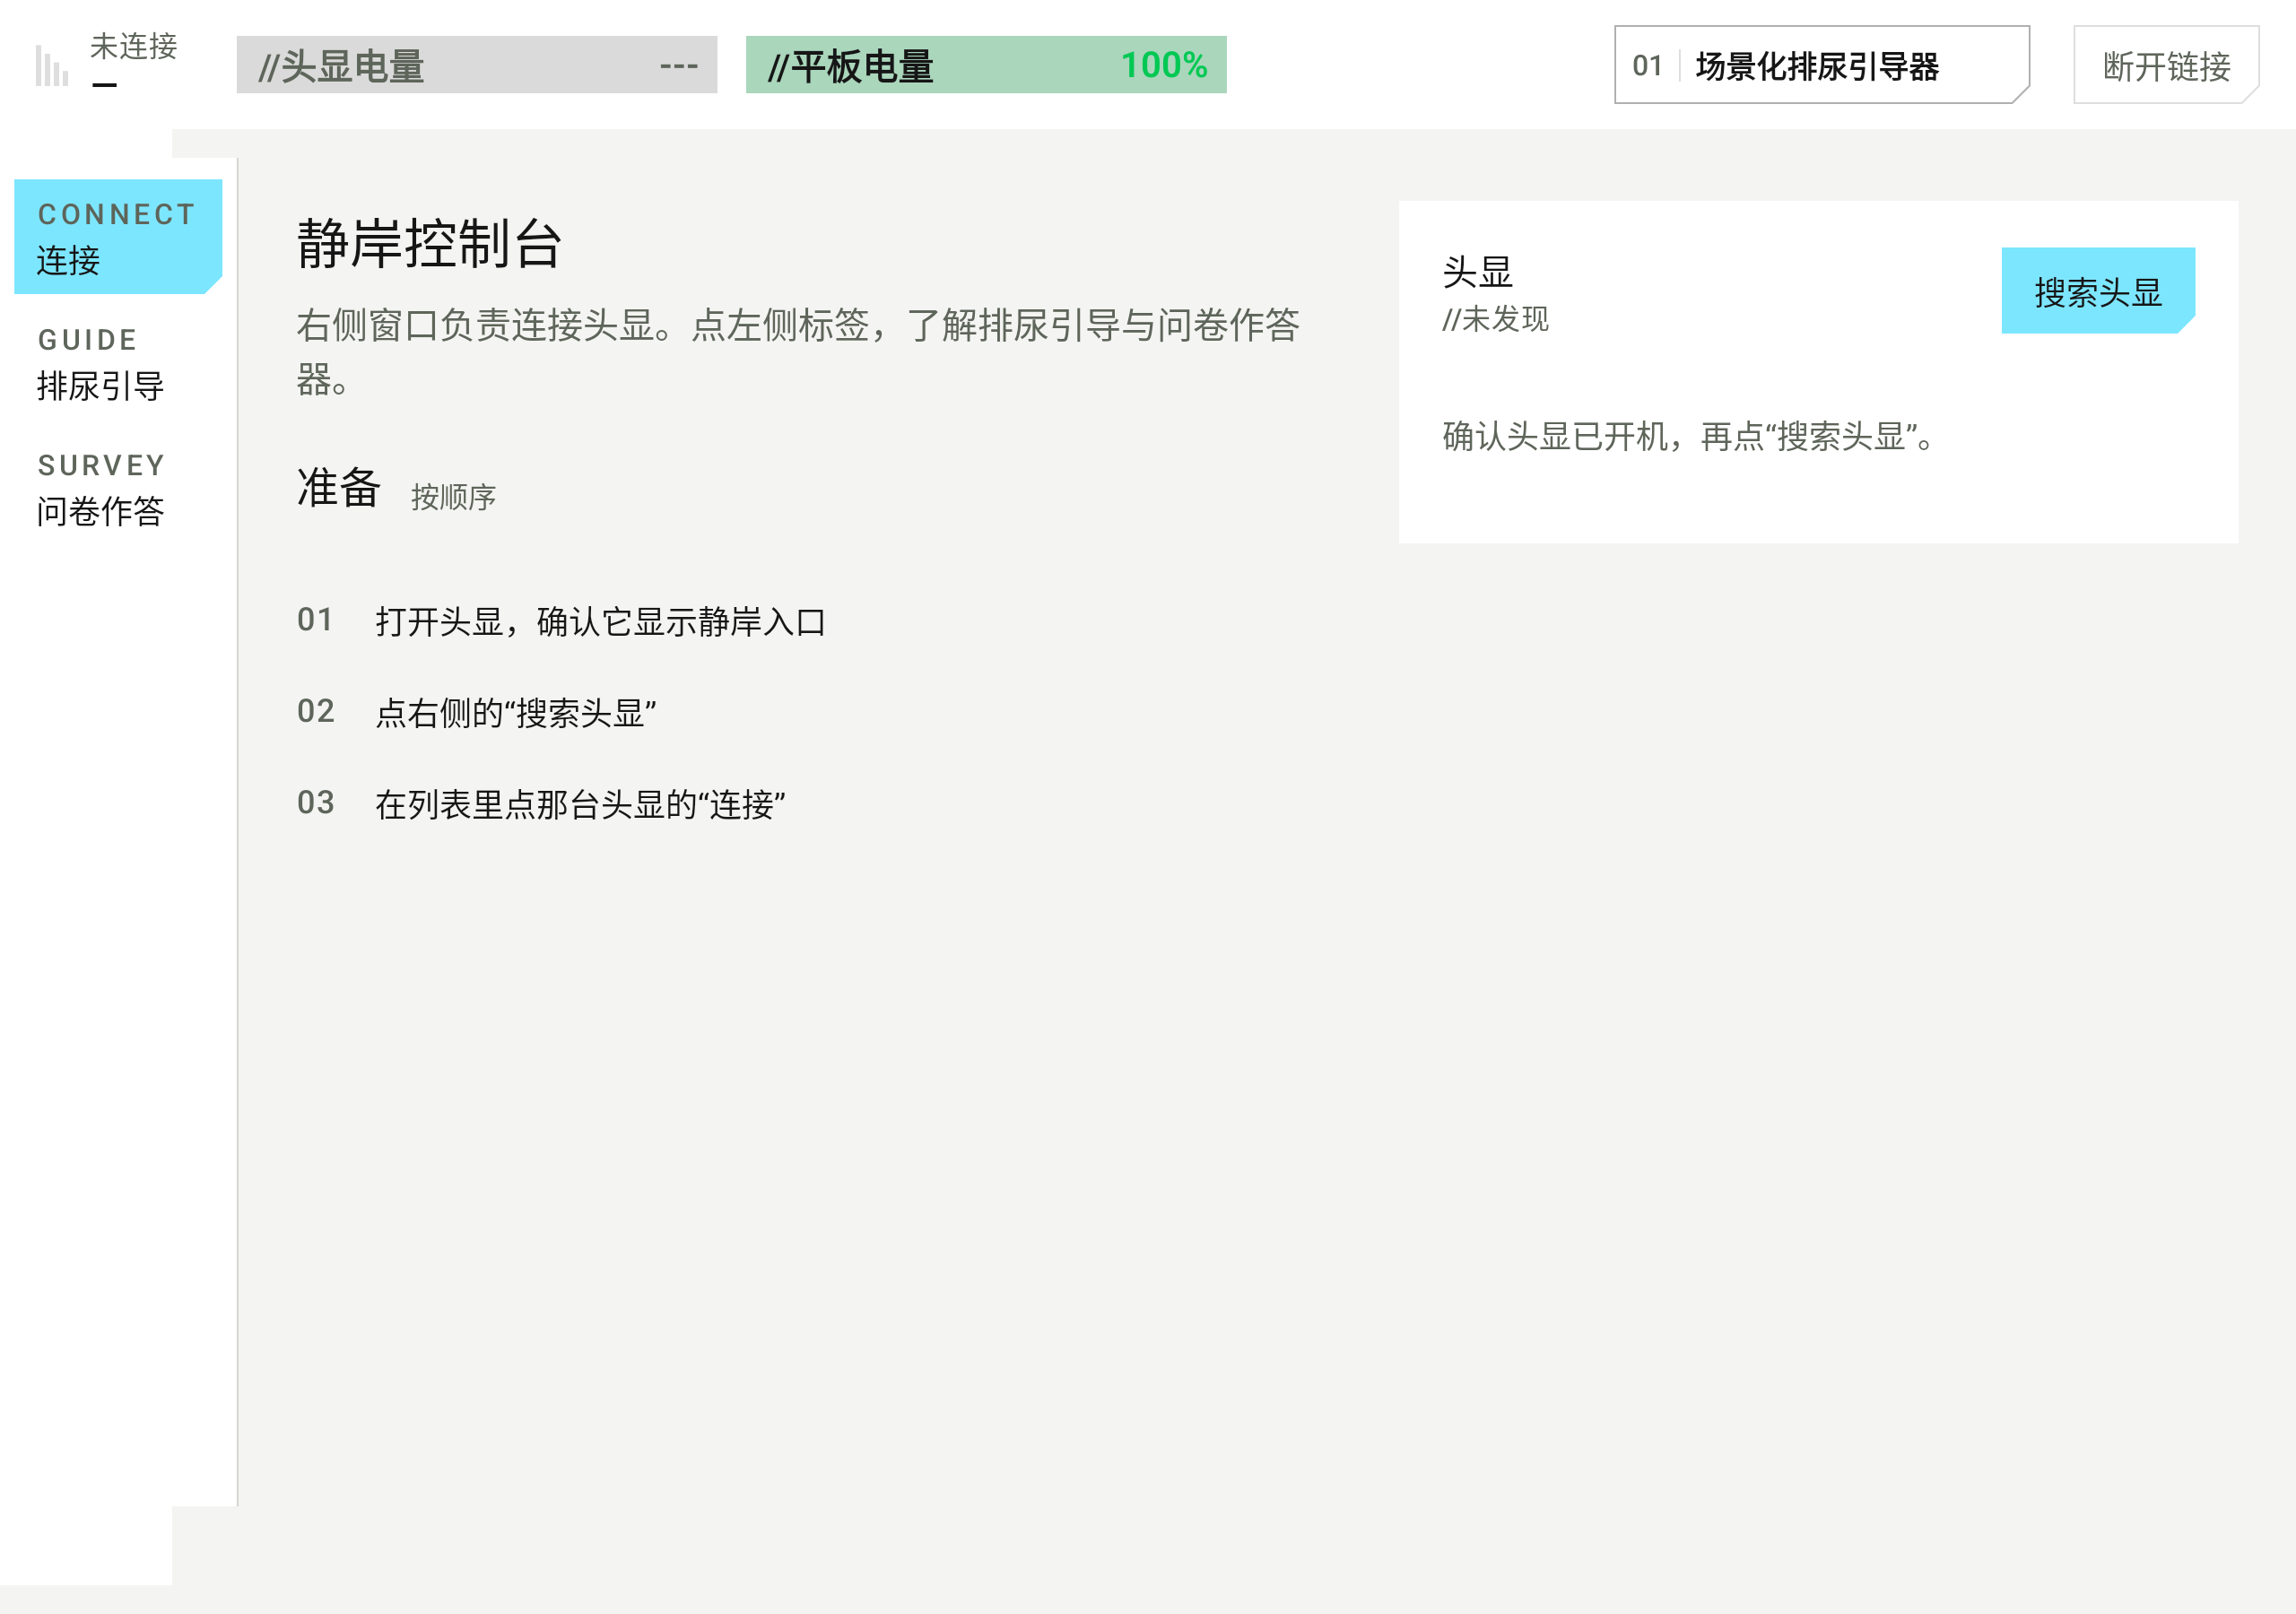
\includegraphics[keepaspectratio]{img/01-connect.png}}

}

\caption{首页：左侧是说明标签，右侧是固定的头显连接窗口。}

\end{figure}%

首页左侧是三个纵向标签，样式与场景化排尿引导器的左侧栏一致：

\begin{itemize}
\tightlist
\item
  \textbf{CONNECT 连接}：连接步骤。
\item
  \textbf{GUIDE 排尿引导}：场景化排尿引导器摘要。
\item
  \textbf{SURVEY 问卷作答}：场景化问卷作答器摘要。
\end{itemize}

标签只用于了解两个应用，不会切换应用。右侧的头显窗口始终留在原位。真正切换应用在顶栏。

\subsection{2.1 连接步骤}\label{ux8fdeux63a5ux6b65ux9aa4}

\begin{enumerate}
\def\labelenumi{\arabic{enumi}.}
\tightlist
\item
  打开头显，确认它显示静岸入口，并停在前台。
\item
  平板右侧点「搜索头显」。
\item
  在「头显」列表里找到设备，点该行的「连接」。
\item
  顶栏出现 \textbf{已连接}，并显示头显与平板的电量。
\end{enumerate}

如果设备被另一台平板占用，先在对方平板上点「断开链接」，再在这台平板上连接。

\begin{figure}[H]

{\centering \pandocbounded{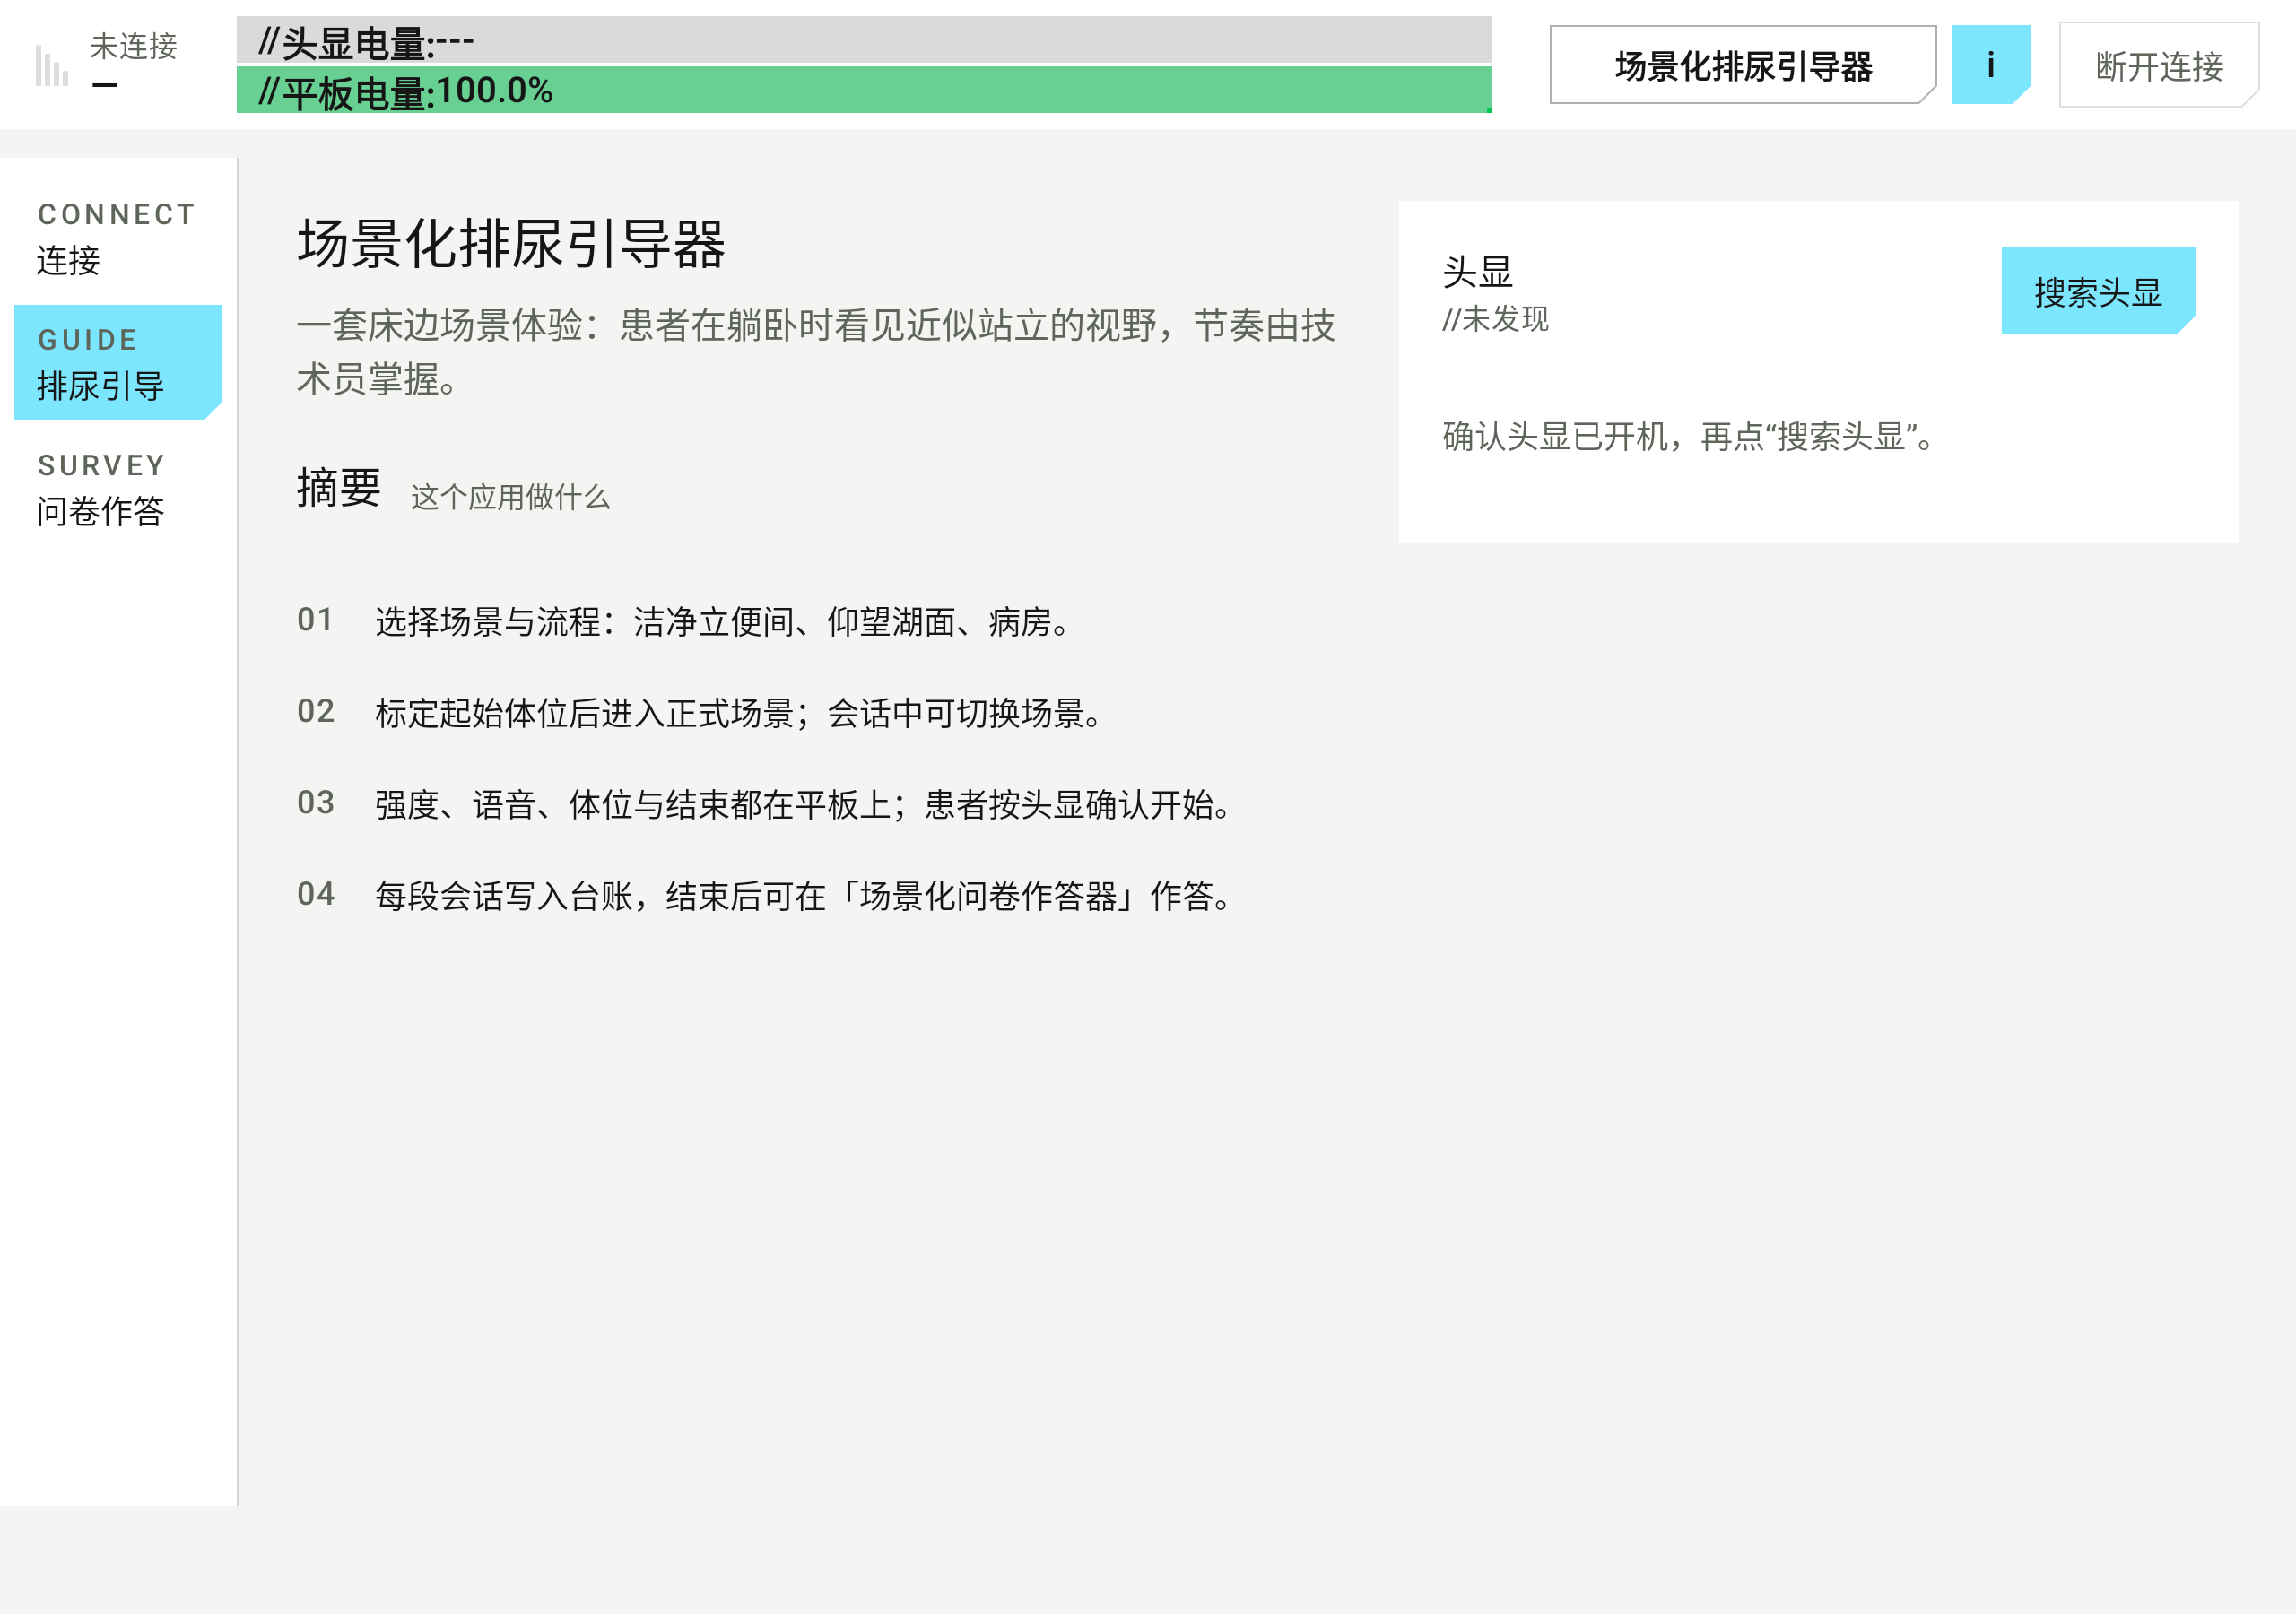
\includegraphics[keepaspectratio]{img/02-guide.png}}

}

\caption{首页的 GUIDE 标签：场景化排尿引导器摘要。}

\end{figure}%

\begin{figure}[H]

{\centering \pandocbounded{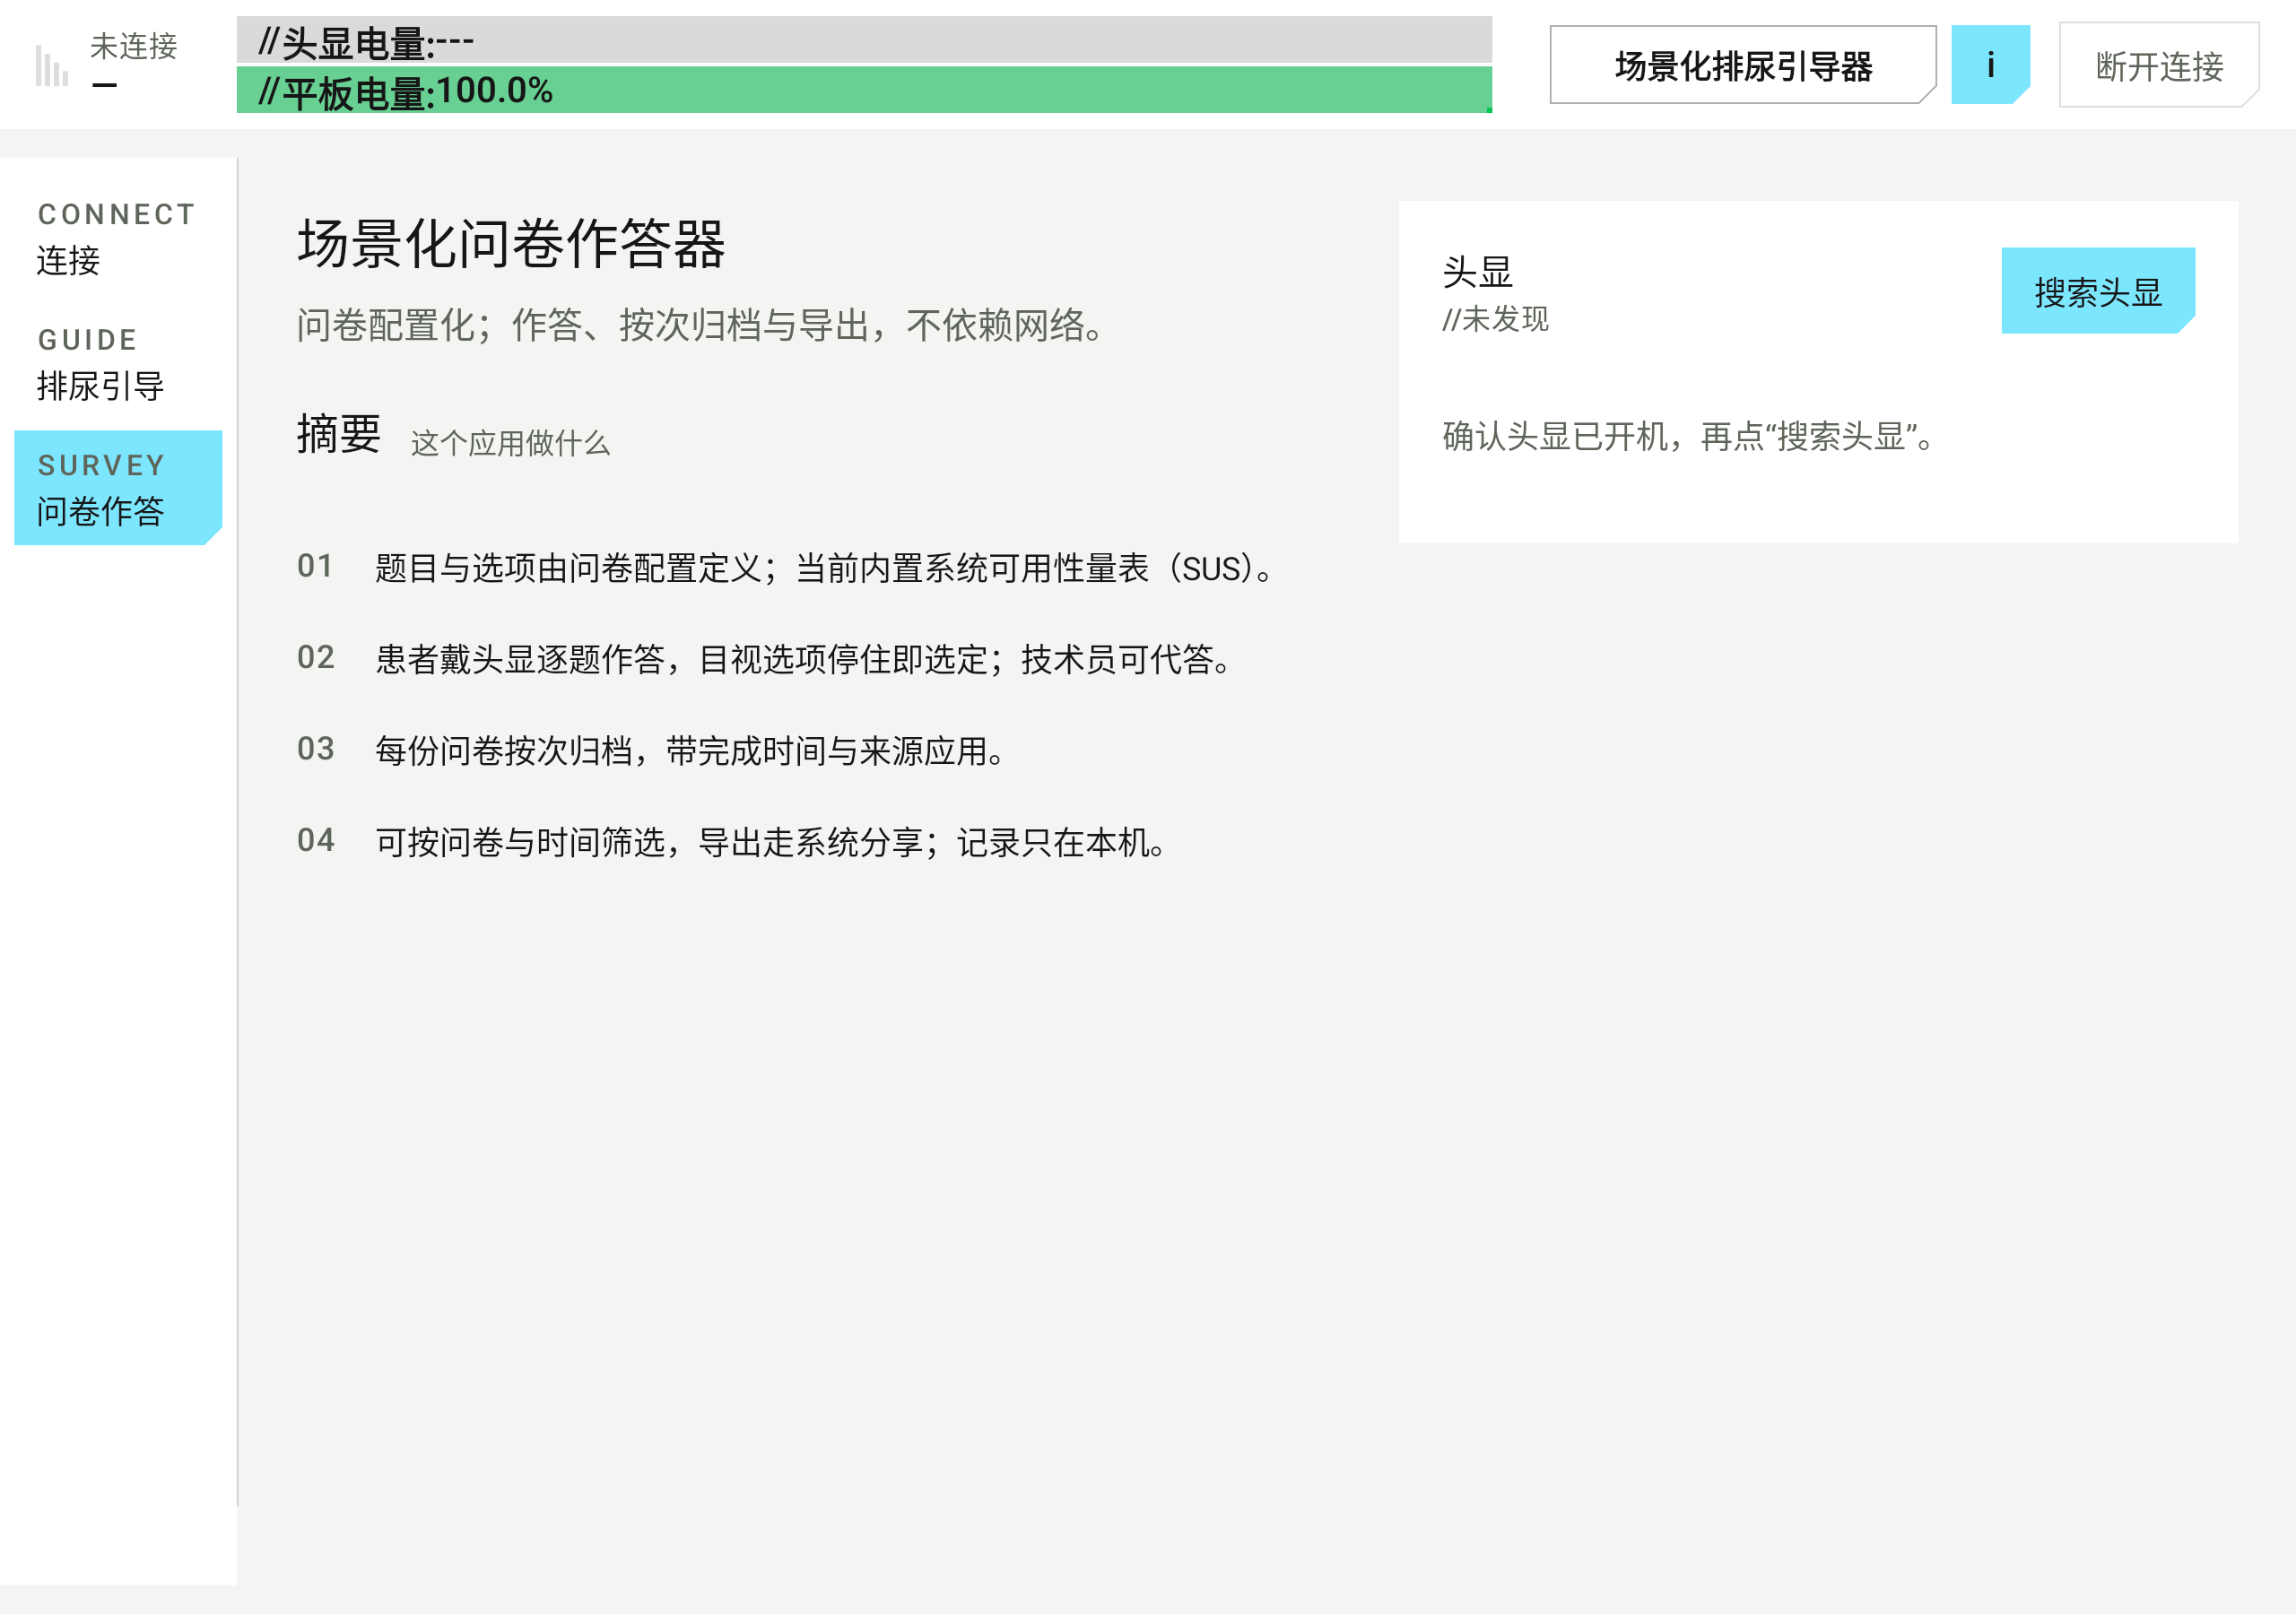
\includegraphics[keepaspectratio]{img/03-survey.png}}

}

\caption{SURVEY 标签：场景化问卷作答器摘要。}

\end{figure}%

\section{3
场景化排尿引导器}\label{ux573aux666fux5316ux6392ux5c3fux5f15ux5bfcux5668}

\subsection{3.1
场景页：准备本次训练}\label{ux573aux666fux9875ux51c6ux5907ux672cux6b21ux8badux7ec3}

\begin{figure}[H]

{\centering \pandocbounded{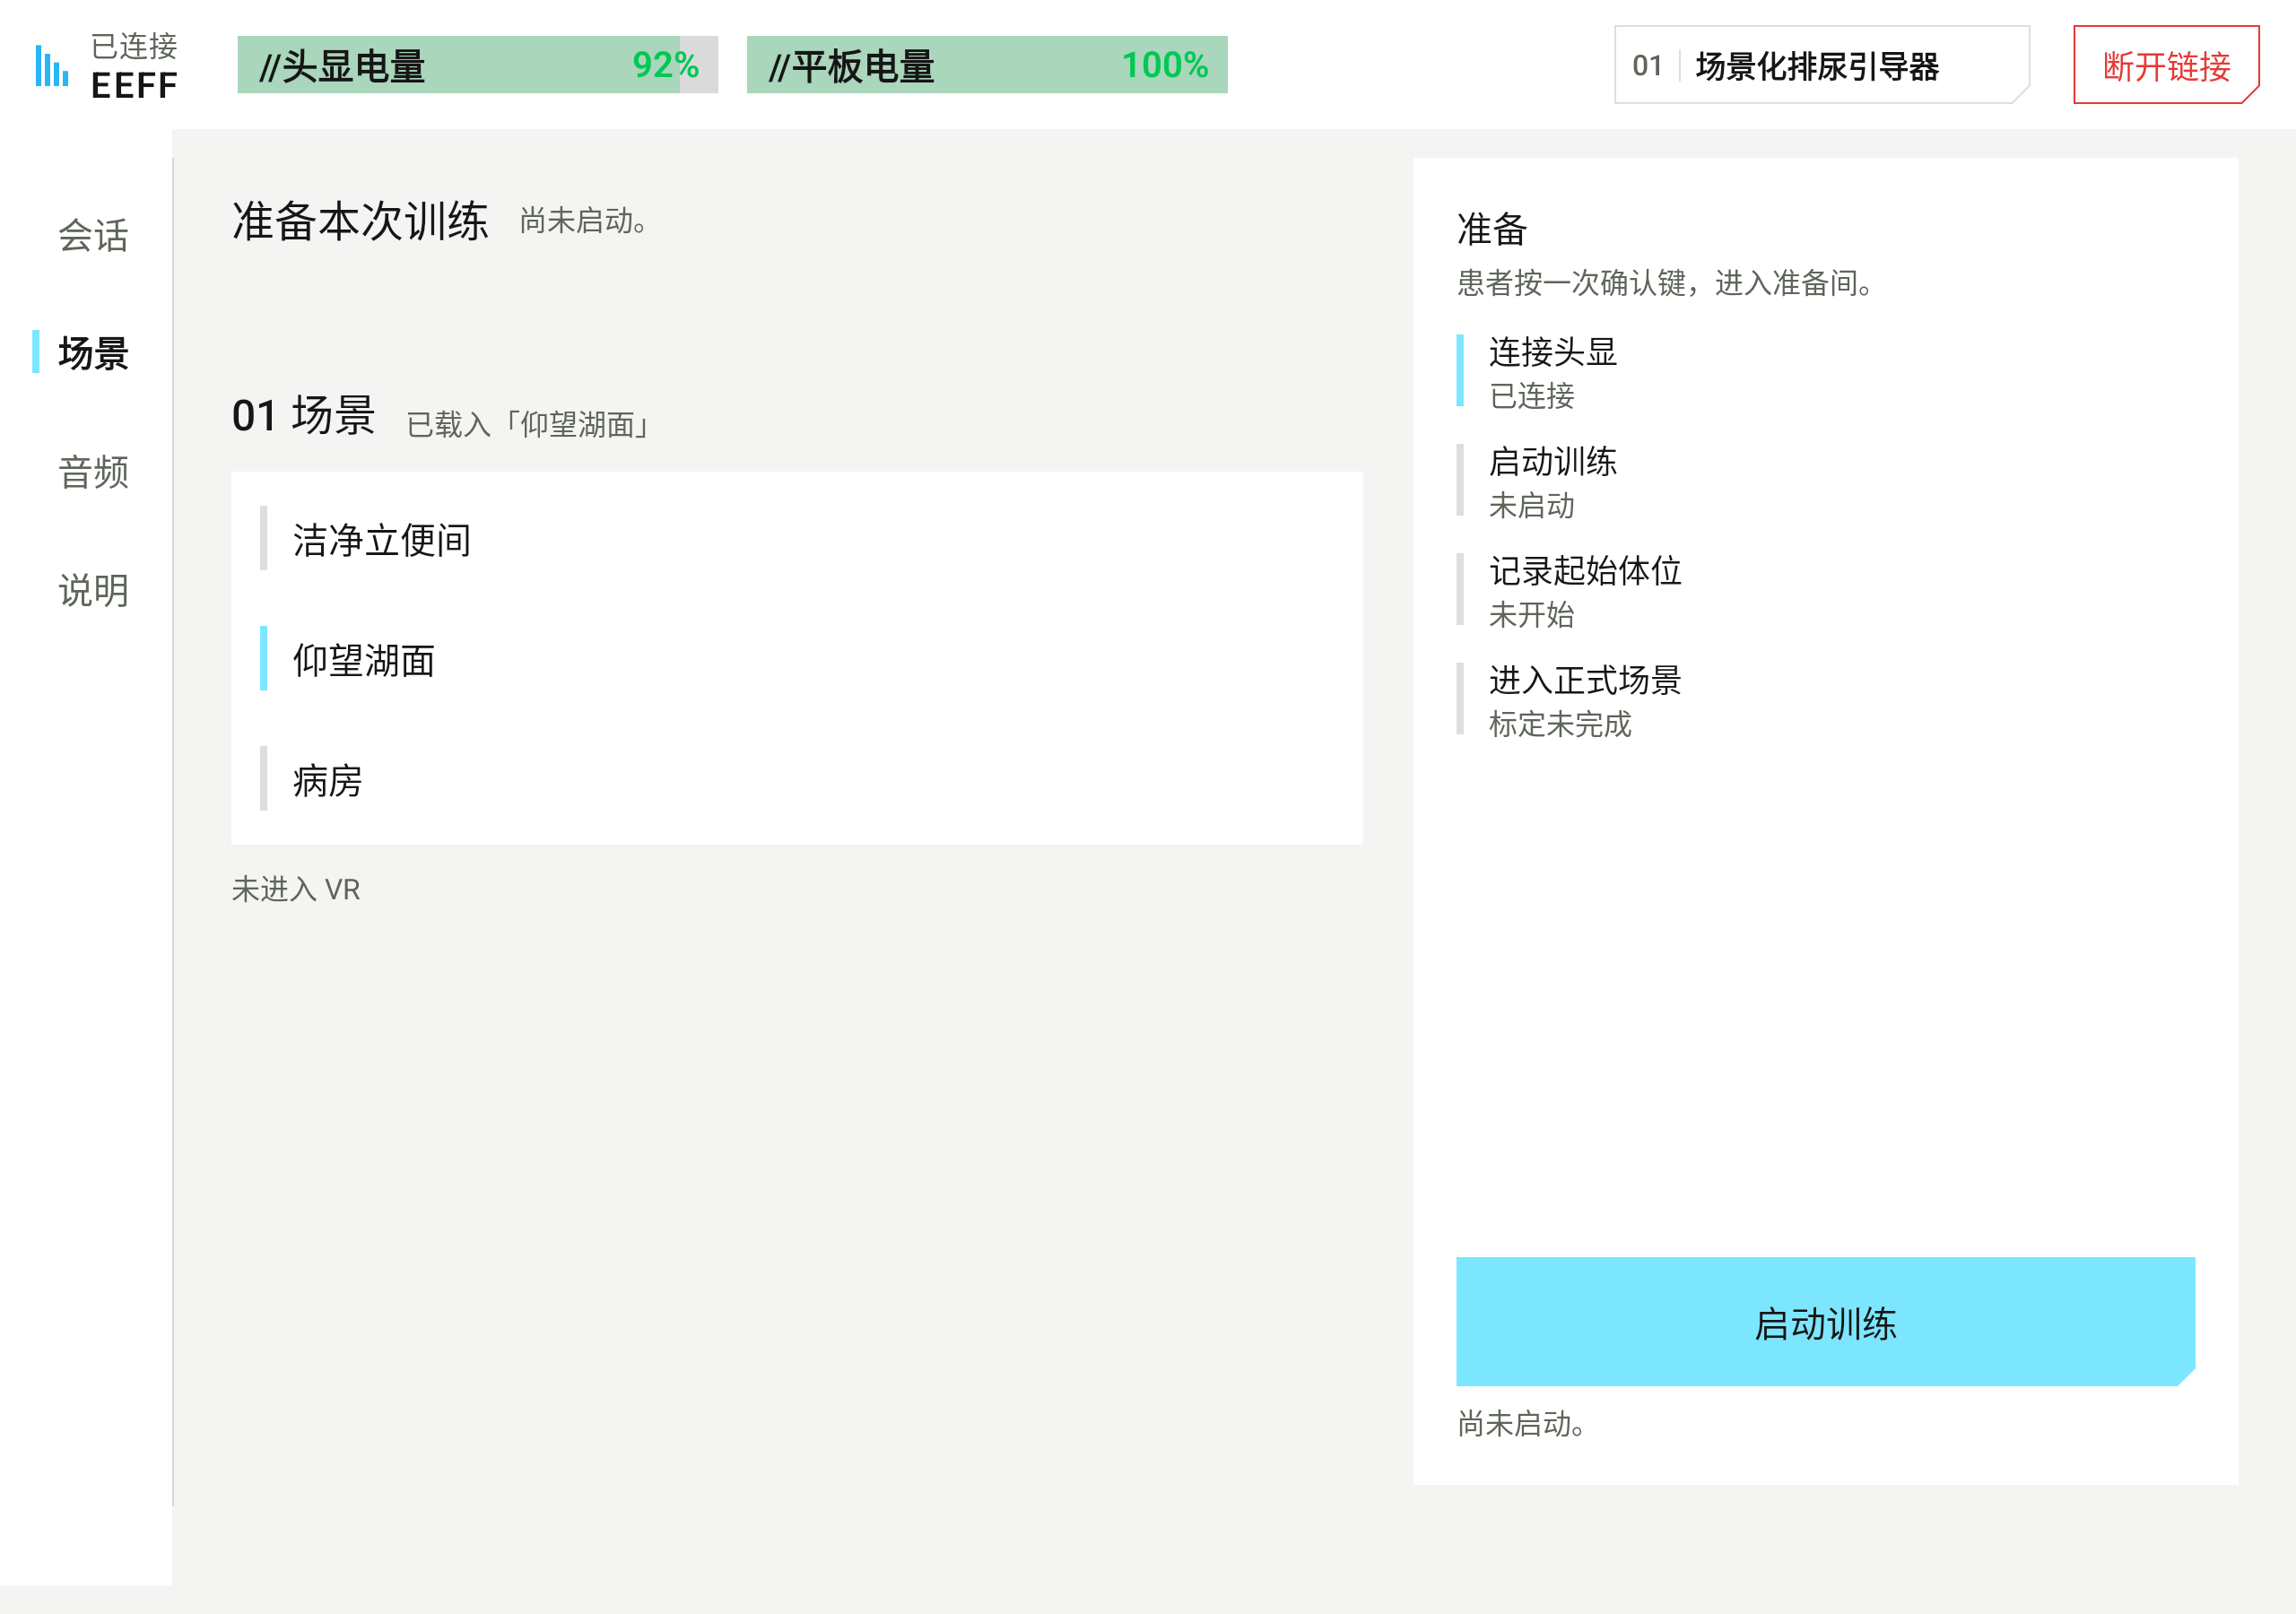
\includegraphics[keepaspectratio]{img/04-bench.png}}

}

\caption{场景页。左侧是场景清单；右侧是启动前的准备链，唯一的主键在链的脚下。}

\end{figure}%

进入应用后默认在 \textbf{场景
页}。会话没开始的时候，这一页只有一件事要做：\textbf{启动}。

\begin{enumerate}
\def\labelenumi{\arabic{enumi}.}
\tightlist
\item
  \textbf{01 场景}：三张正式场景的清单。

  \begin{itemize}
  \tightlist
  \item
    \textbf{洁净立便间}：站立视角，目标是站立排尿。
  \item
    \textbf{仰望湖面}：平躺、抬头看天时最自然。
  \item
    \textbf{病房}：仰卧视角，目标是安静地看着天花板与监护仪。
  \item
    标定完成前它们只列出名字，不能点；页头写明当前载入的是哪一个。
  \end{itemize}
\item
  \textbf{右侧「准备」}：连接头显 → 启动训练 → 记录起始体位 →
  进入正式场景，四步成链；链的脚下就是「启动训练」，那是这一页唯一的按钮。
\end{enumerate}

\subsection{3.2 启动与标定}\label{ux542fux52a8ux4e0eux6807ux5b9a}

{\def\LTcaptype{none} % do not increment counter
\begin{longtable}[]{@{}
  >{\raggedright\arraybackslash}p{(\linewidth - 4\tabcolsep) * \real{0.3333}}
  >{\raggedright\arraybackslash}p{(\linewidth - 4\tabcolsep) * \real{0.3333}}
  >{\raggedright\arraybackslash}p{(\linewidth - 4\tabcolsep) * \real{0.3333}}@{}}
\toprule\noalign{}
\begin{minipage}[b]{\linewidth}\raggedright
步
\end{minipage} & \begin{minipage}[b]{\linewidth}\raggedright
动作
\end{minipage} & \begin{minipage}[b]{\linewidth}\raggedright
说明
\end{minipage} \\
\midrule\noalign{}
\endhead
\bottomrule\noalign{}
\endlastfoot
1 & 右侧点「启动训练」 & 头显页面被拉起 \\
2 & 患者按一次头显右侧按钮进入画面 & 这是浏览器强制手势；20
秒未按会重开页面 \\
3 & 患者进入准备间 & 调整躺姿与头显位置 \\
4 & 技术员点「记录起始体位」 & 记录期间世界静止，患者保持不动 \\
5 & 场景卡解锁，选卡后点「进入正式场景」 & 校准帧保留，只换世界内容 \\
6 & 填「时长」，点「修正 · 起身」 & 整数秒 4--20，默认
10；正反两个方向同速 \\
\end{longtable}
}

\subsection{3.3 会话中}\label{ux4f1aux8bddux4e2d}

\begin{figure}[H]

{\centering \pandocbounded{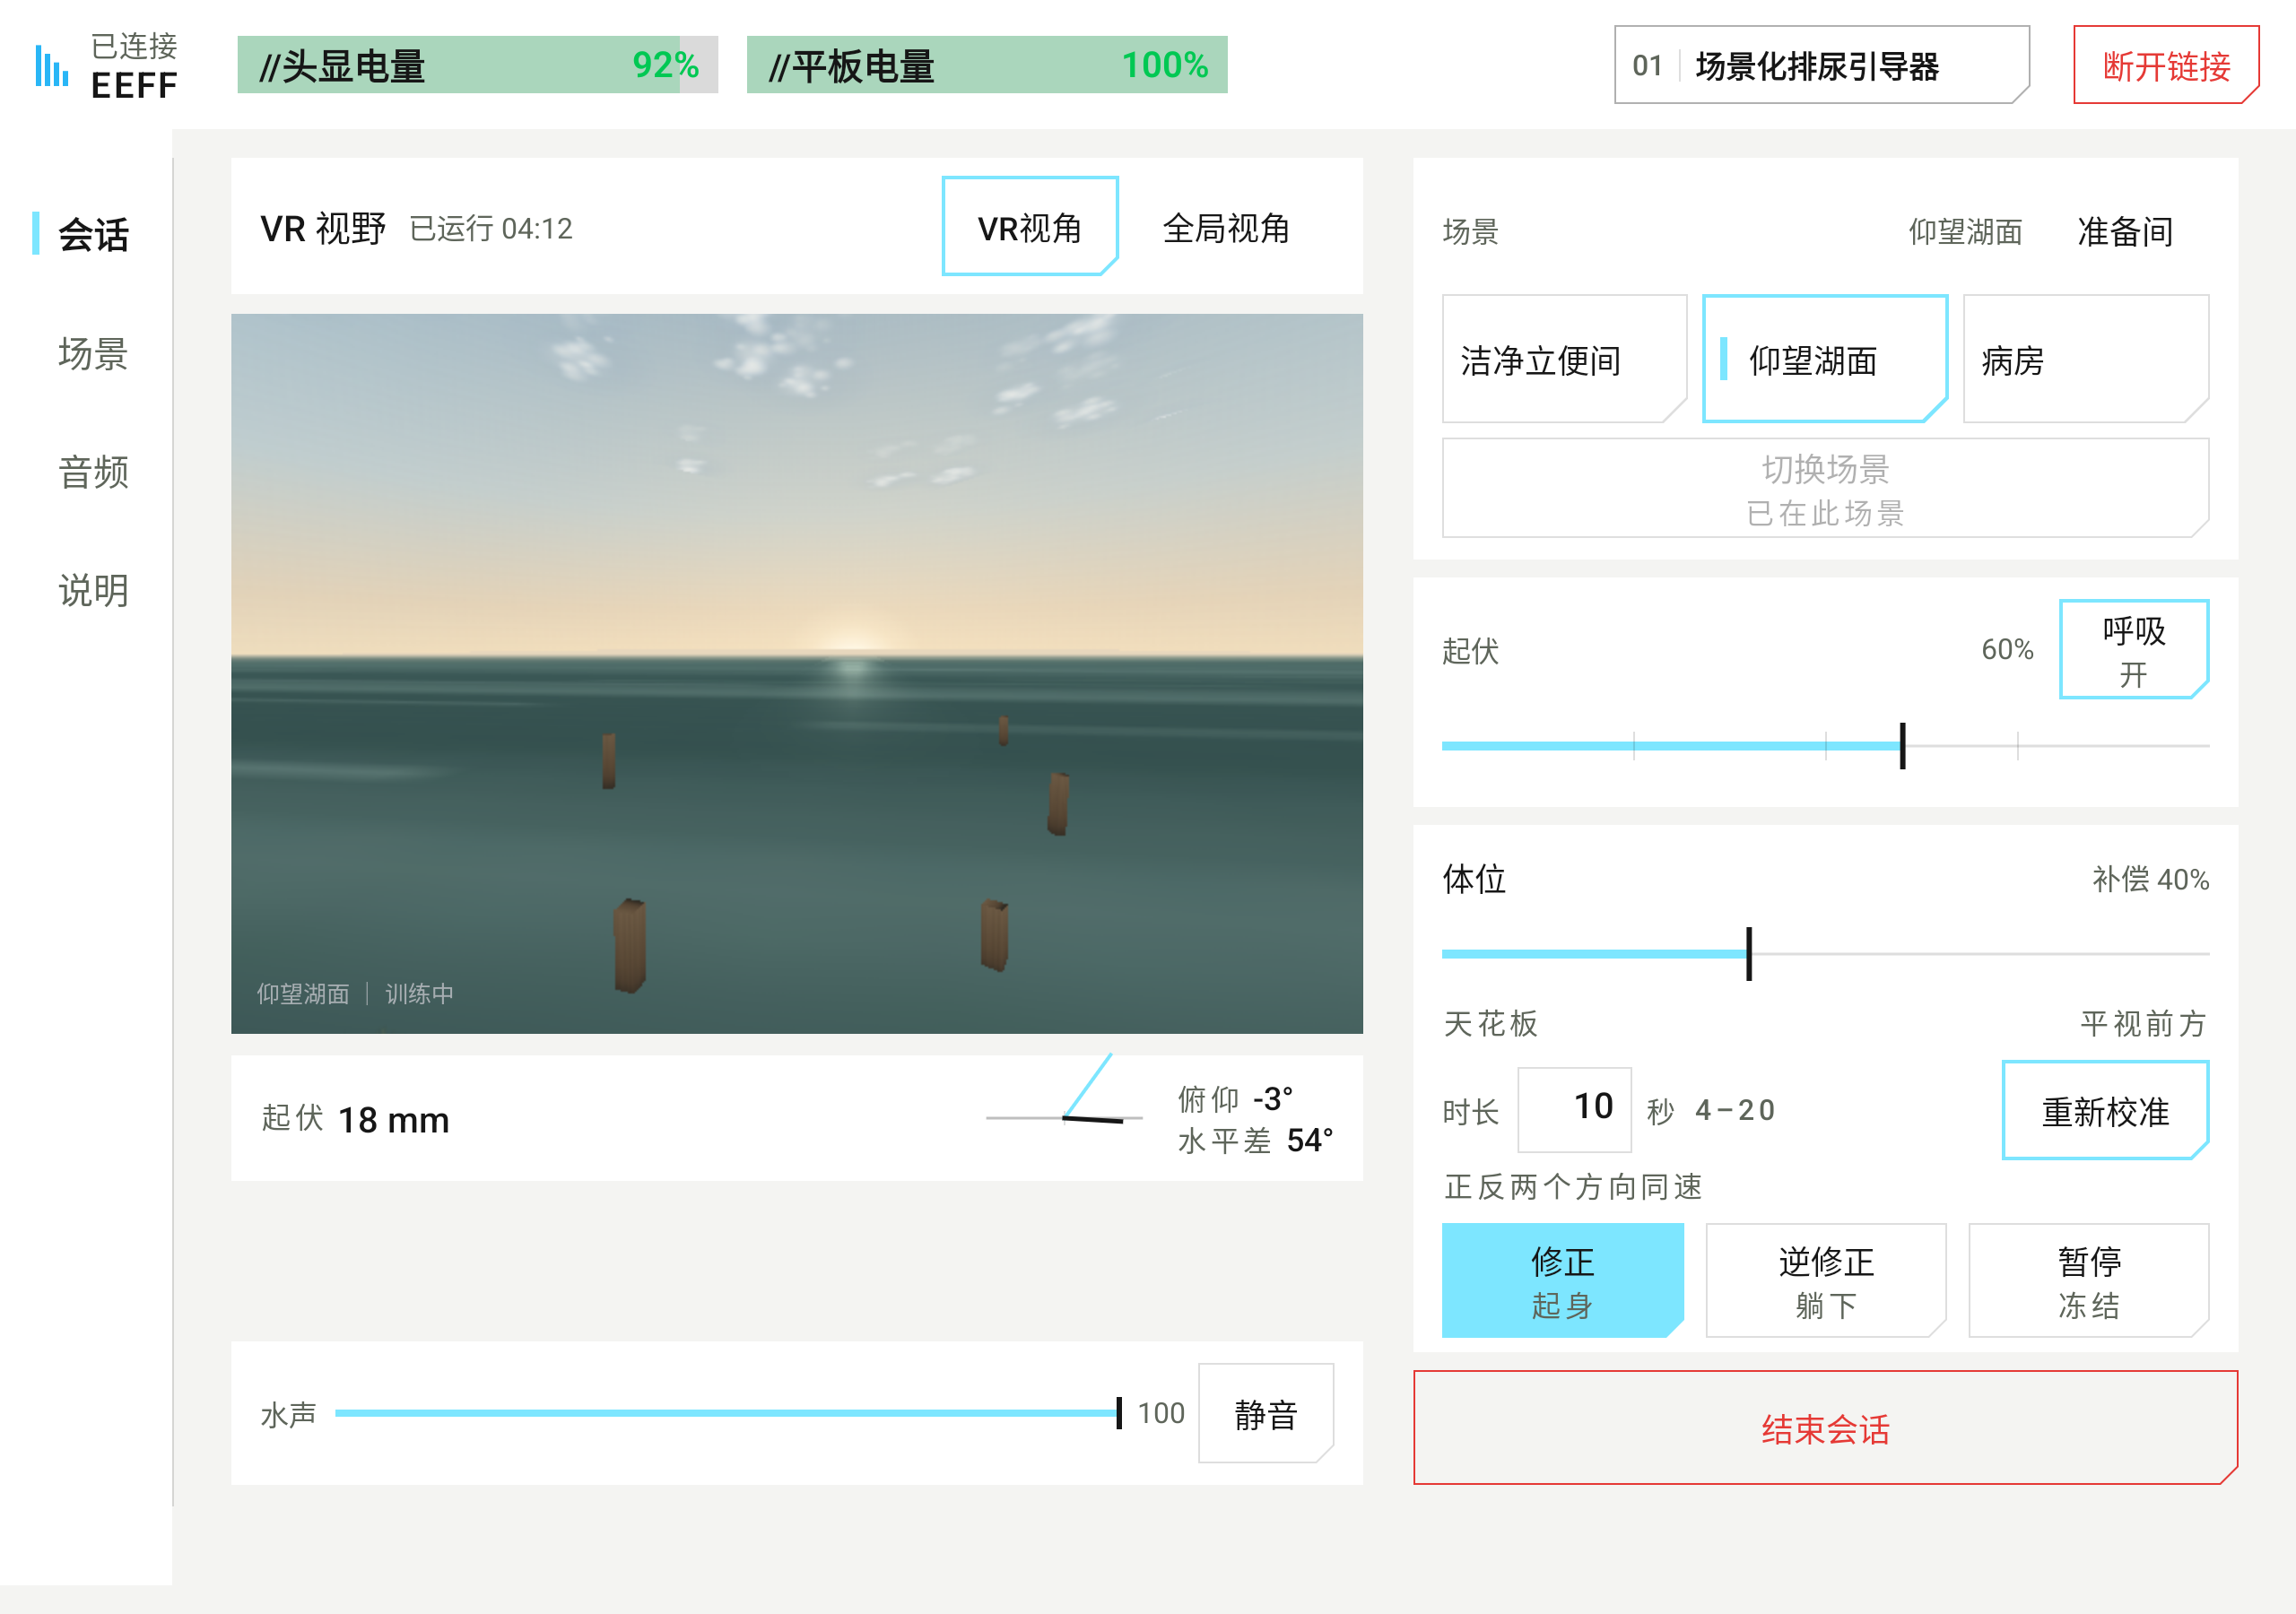
\includegraphics[keepaspectratio]{img/05-session.png}}

}

\caption{会话页。标题卡、患者画面、读数卡与水声卡在左列；场景、起伏、体位与结束在右列。}

\end{figure}%

左列从上到下：标题卡 → 患者画面（占三分之二）→ 读数卡 →
水声卡。右列三块：场景、起伏、体位。

\begin{itemize}
\tightlist
\item
  \textbf{标题卡}：\texttt{VR\ 视野} 是头显当前画面，\texttt{全局视角}
  是操作员俯瞰；右侧是本次会话时钟。
\item
  \textbf{患者画面}：镜像，约两秒延迟之内跟手。
\item
  \textbf{读数卡}：\texttt{起伏} 是当前竖直位移；旁边的小盘画两条水平线
  ------
  灰的是患者身下真实世界的水平，冰蓝的是场景被放进去的水平。\textbf{两条线的夹角就是还没补偿完的角度}，右侧写作「水平差」。盘上的墨针是患者头部的实际俯仰。
\item
  \textbf{水声}：一条 0--100 的音量条和「静音」。只关水声，不动语音。
\item
  \textbf{场景}：会话中可换场景。先点卡片选中，再点「切换场景」执行；选中的就是当前场景时按钮置灰并写「已在此场景」。页头的「准备间」把人送回中性空房（见下）。
\item
  \textbf{起伏}：0--100\%
  的滑条，「呼吸」开关决定这份起伏是自然呼吸还是等幅机械。场景可以声明自己不动，那时这一行显示「本场景无起伏」。
\item
  \textbf{体位}：一条滑条 + 一个「时长」+ 三个键。

  \begin{itemize}
  \tightlist
  \item
    滑条左端是「天花板」（患者的真实俯仰），右端是「平视前方」（场景声明的前方）。\textbf{按下滑条就是接管}：正在跑的斜坡与视线动画会停在原地，之后由手的移动决定目标，页面按自己的限速跟随，不会瞬移。填充是页面已施加的值，竖线是手指的位置。
  \item
    「时长」是斜坡长度，正反同速。
  \item
    「修正 · 起身」「逆修正 · 躺下」「暂停」：暂停把斜坡就地冻结。
  \end{itemize}
\item
  \textbf{重新校准}：在「时长」右侧。需要重做起始体位时用；它跳过稳定等待，直接进入
  3 秒取样。
\item
  \textbf{结束会话}：页面底部整宽的红色细框键。
\end{itemize}

\textbf{换场会有约四分之一秒的黑幕}：淡到黑、换内容、淡回。声音随场景切换；尽量在语音之间换场，别在一句话中途切。

\subsection{3.3.1 回到准备间}\label{ux56deux5230ux51c6ux5907ux95f4}

点场景块页头的「准备间」，再确认切换，就会回到开场那间灰房：

\begin{itemize}
\tightlist
\item
  水声、语音、起伏一起停；世界按场景声明回到「真实天花板」，眼位也回床上。
\item
  \textbf{会话不会结束}，时钟继续走；台账里这一段记为独立的一段。
\item
  校准帧保留，所以从准备间再进正式场景不需要重新标定。
\end{itemize}

这个房间的用途是''停一下''：患者需要缓一缓、要换体位、或者技术员想先收走声音再说话。

\subsection{3.4 语音页}\label{ux8bedux97f3ux9875}

\begin{figure}[H]

{\centering \pandocbounded{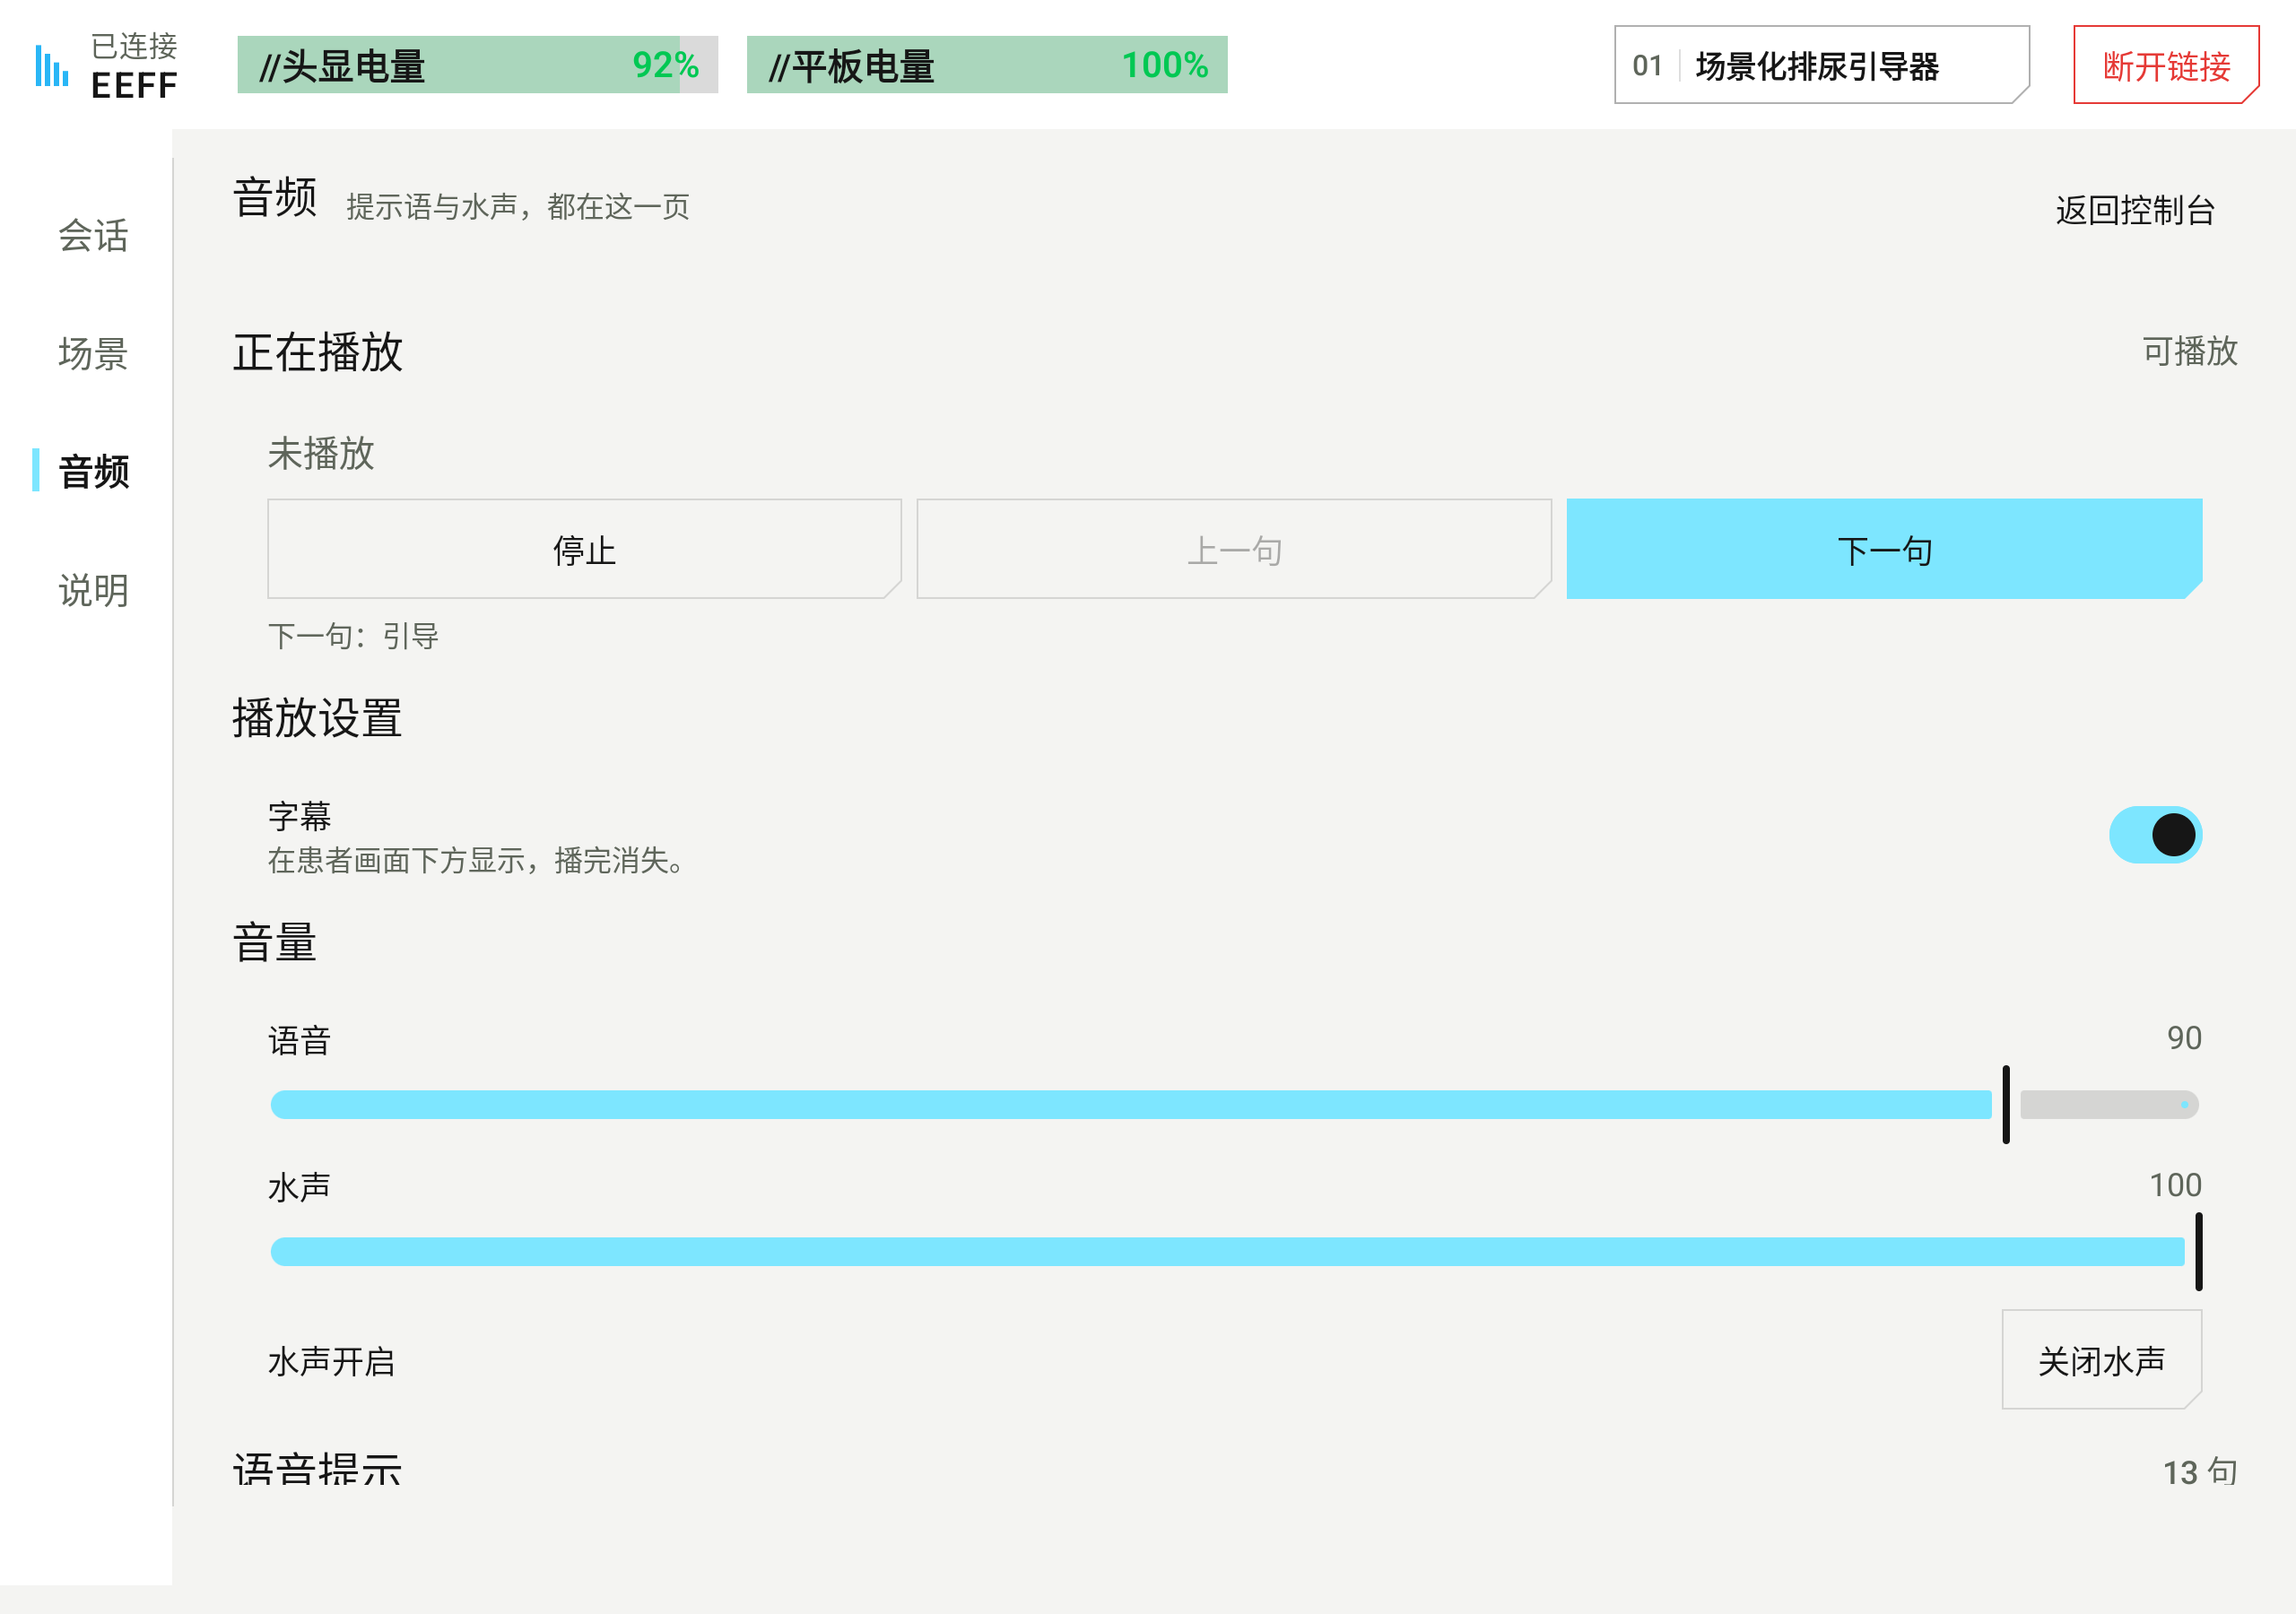
\includegraphics[keepaspectratio]{img/06-voice.png}}

}

\caption{语音页：播放状态、字幕、声音、连续播放与音色。}

\end{figure}%

\begin{itemize}
\tightlist
\item
  \textbf{正在播放}：显示当前句；可「停止」或「下一句」。
\item
  \textbf{字幕}：在患者画面下方显示，播完消失。
\item
  \textbf{连续播放}：开始 / 想象 / 放松 / 收束，一次运行整段脚本。
\item
  \textbf{音色}：女声 / 男声；切换会短暂停顿。
\item
  \textbf{声音}：水声开关、语音音量、水声压低级数。
\item
  \textbf{语音提示}：按组展开单句清单，逐句播放。
\end{itemize}

语音播放时环境声自动压低 12
dB。问卷题干的朗读开关在场景化问卷作答器里，不在训练语音页。

\subsection{3.5 体验记录}\label{ux4f53ux9a8cux8bb0ux5f55}

左栏新增 \textbf{体验} 页，用于会话结束后的床边访谈。

\begin{enumerate}
\def\labelenumi{\arabic{enumi}.}
\tightlist
\item
  点「填写体验表」。场景、日期与会话时长自动带入，不需要手填。
\item
  受试者编号可选；不填则记录为匿名。
\item
  八项 0--10
  评分：失重强度、方向感错乱、场景真实感、身体对齐、舒适度、头晕、恶心、再次体验意愿。
\item
  漂浮方向四选一：上升、下沉、漂浮、无明显方向。
\item
  备注可选，可记录患者原话、体位或设备异常。
\item
  点「保存记录」。记录立即出现在下方列表，可展开查看全部字段。
\item
  点「导出 CSV」生成表格文件，UTF-8 BOM，中文列名，可直接用 Excel 打开。
\end{enumerate}

CSV 一行一份体验记录。受试者编号和备注允许为空，其余评分按 0--10 归档。

\subsection{3.6 结束与断开}\label{ux7ed3ux675fux4e0eux65adux5f00}

\begin{enumerate}
\def\labelenumi{\arabic{enumi}.}
\tightlist
\item
  会话页底部点「结束会话」。
\item
  画面淡出，头显结束会话；平板保留本次记录。
\item
  帮患者摘头显，先让其躺一会儿再起身。
\end{enumerate}

\textbf{结束会话}是正常停止。\textbf{断开链接}是急停：头显立即冻结，等待
5 秒重连；5 秒内没有连回，头显退出场景回到首页。

患者不操作头显。患者说停或直接取下头显时，技术员在平板点「结束会话」。本版本没有独立急停按钮。

\section{4
场景化问卷作答器}\label{ux573aux666fux5316ux95eeux5377ux4f5cux7b54ux5668}

会话结束后，在顶栏把应用切到「场景化问卷作答器」。会话进行中不能切换。

\subsection{4.1 作答}\label{ux4f5cux7b54}

\begin{figure}[H]

{\centering \pandocbounded{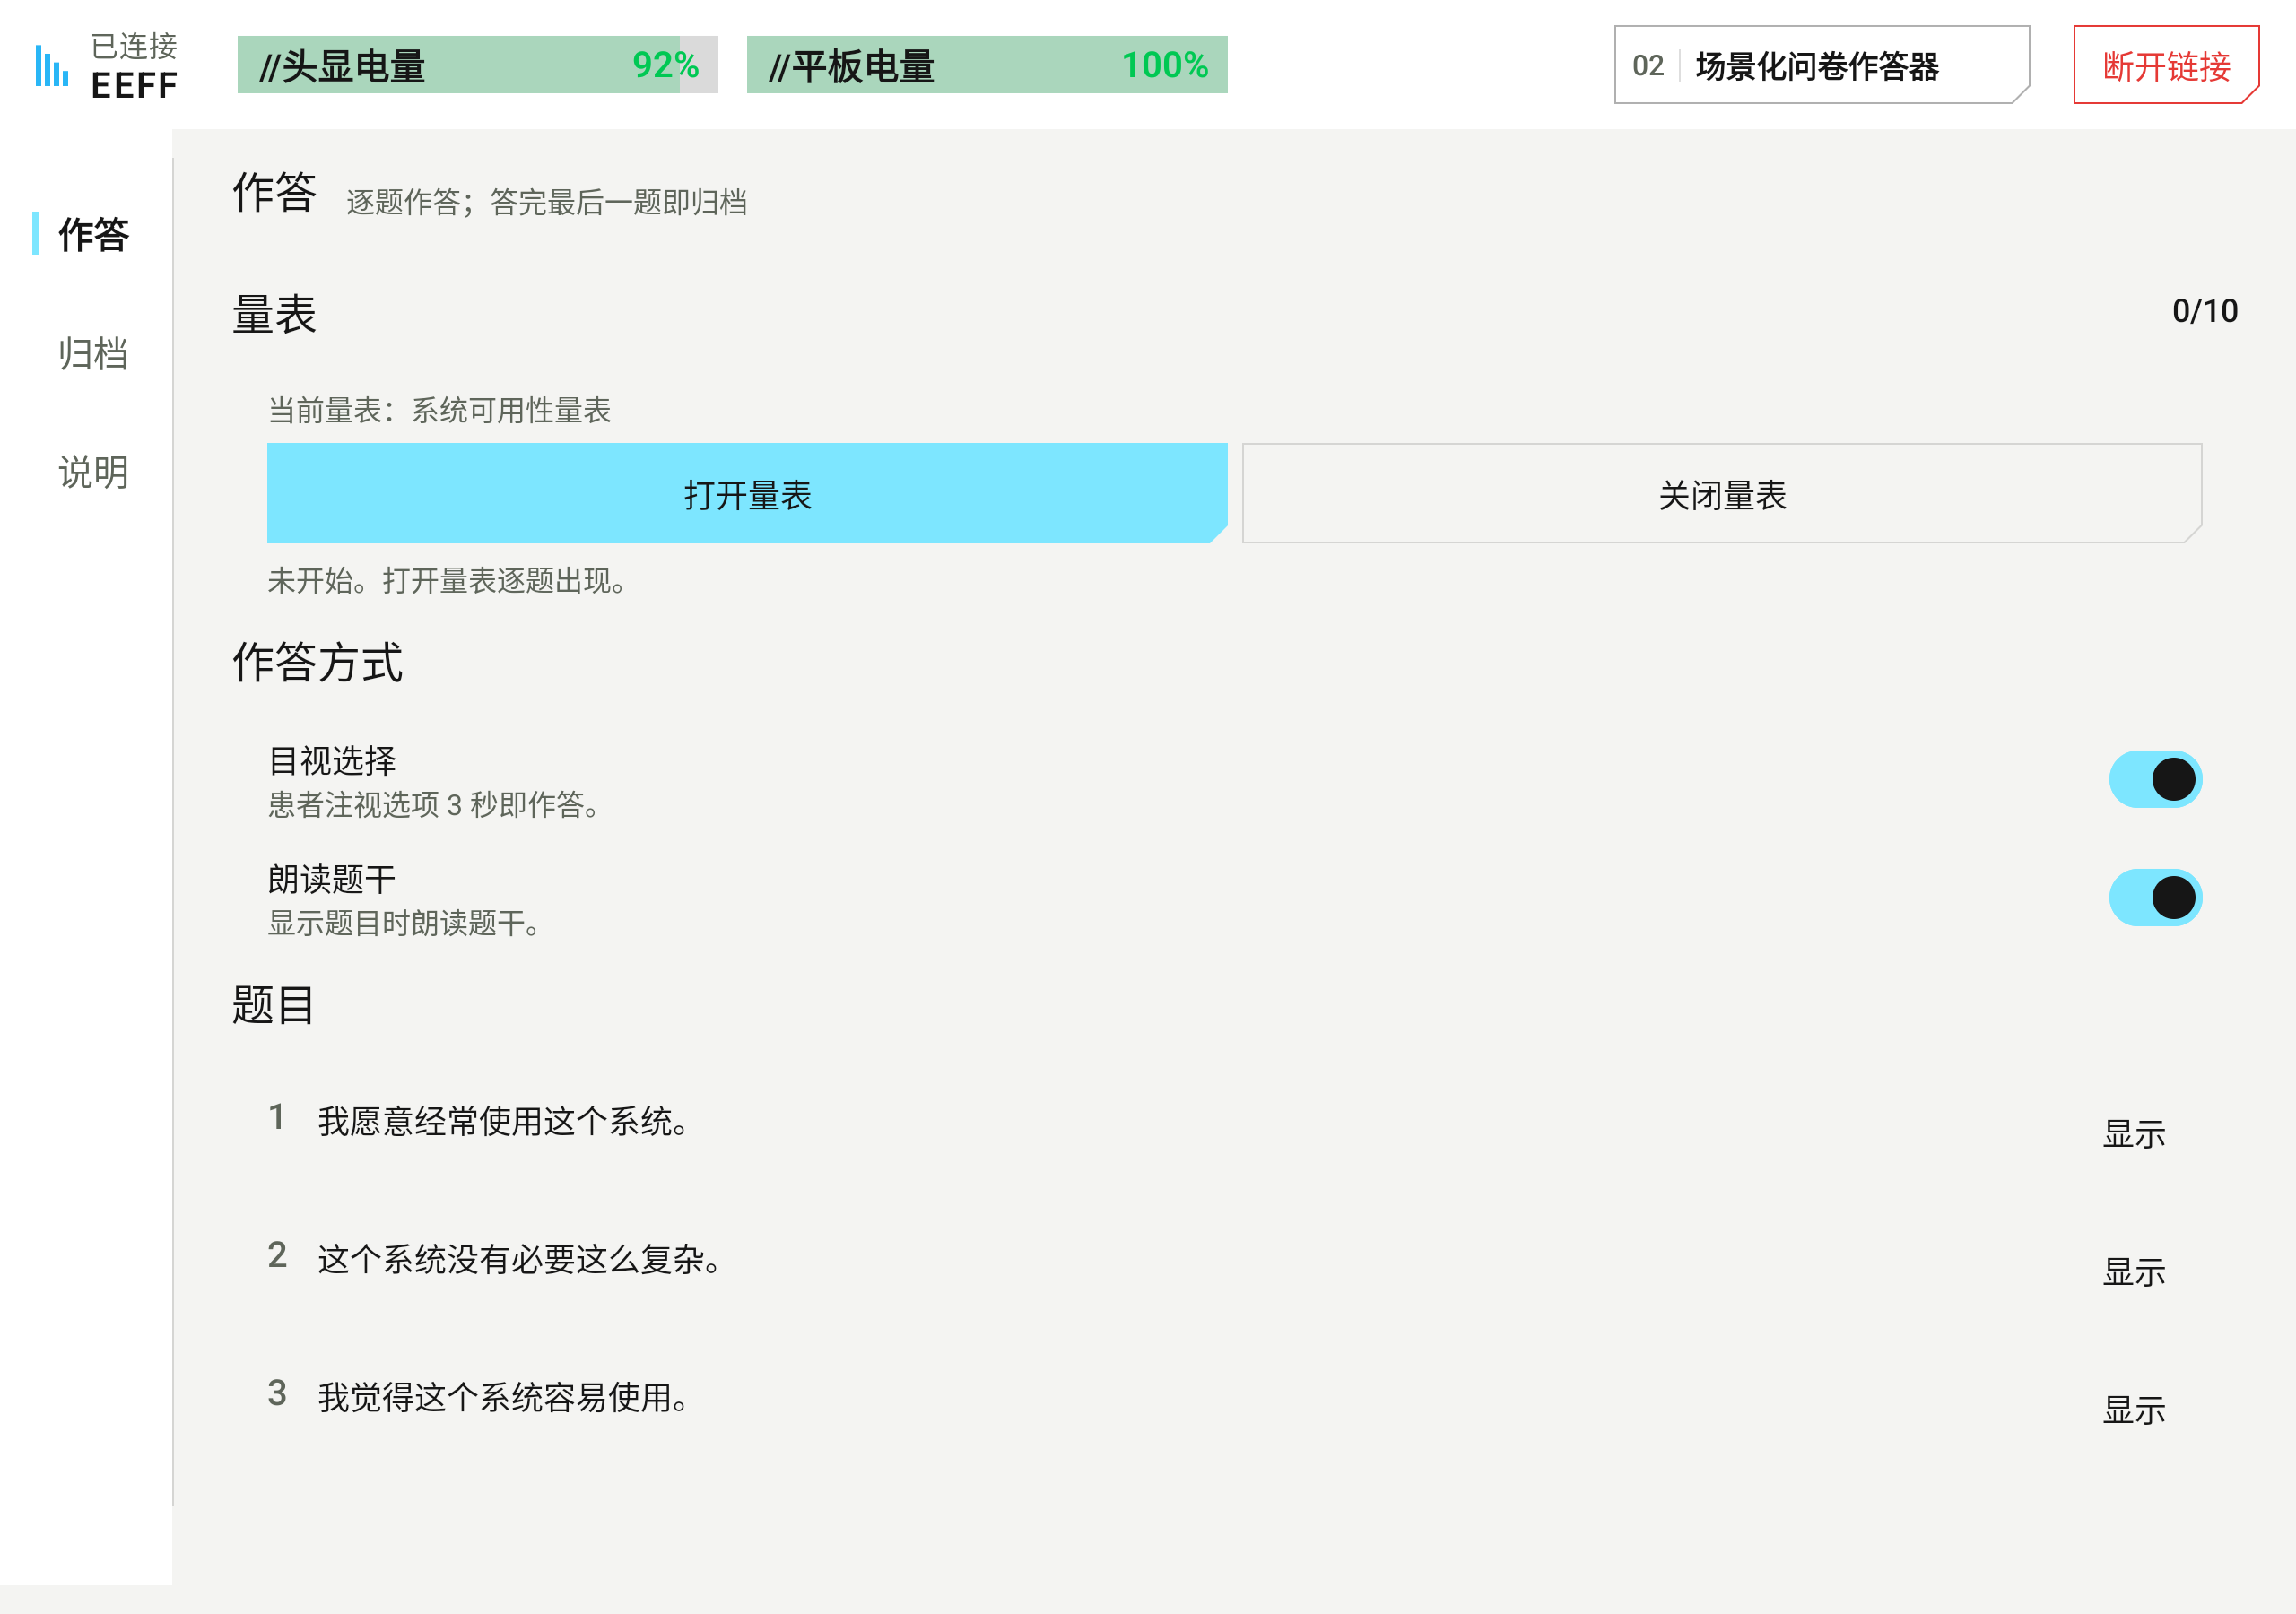
\includegraphics[keepaspectratio]{img/07-questionnaire.png}}

}

\caption{场景化问卷作答器。左侧 作答 / 归档 / 说明
三栏；作答页先显示当前量表，再是开关、作答方式与题目。}

\end{figure}%

进入后左侧是 \textbf{作答}、\textbf{归档}、\textbf{说明}
三栏，和排尿引导的左侧栏同构。作答页：

\begin{enumerate}
\def\labelenumi{\arabic{enumi}.}
\tightlist
\item
  「当前量表」先写明本次加载的问卷；本版本内置
  \textbf{系统可用性量表（SUS）}。
\item
  点「打开量表」，题目出现在头显里。
\item
  患者目视选项，停住约 3 秒即选定；技术员也可以在平板上按 1--5 代答。
\item
  「朗读题干」在题目出现时同步播放该题语音。
\item
  答完最后一题即记录；中途关闭只保存已完成的部分。
\end{enumerate}

量表切换是下一版的骨架：题目与选项来自问卷配置，新增量表时增加配置与对应语音资源，作答页会显示新的当前量表；作答与归档的入口不变。

\subsection{4.2
归档、筛选与导出}\label{ux5f52ux6863ux7b5bux9009ux4e0eux5bfcux51fa}

\begin{figure}[H]

{\centering \pandocbounded{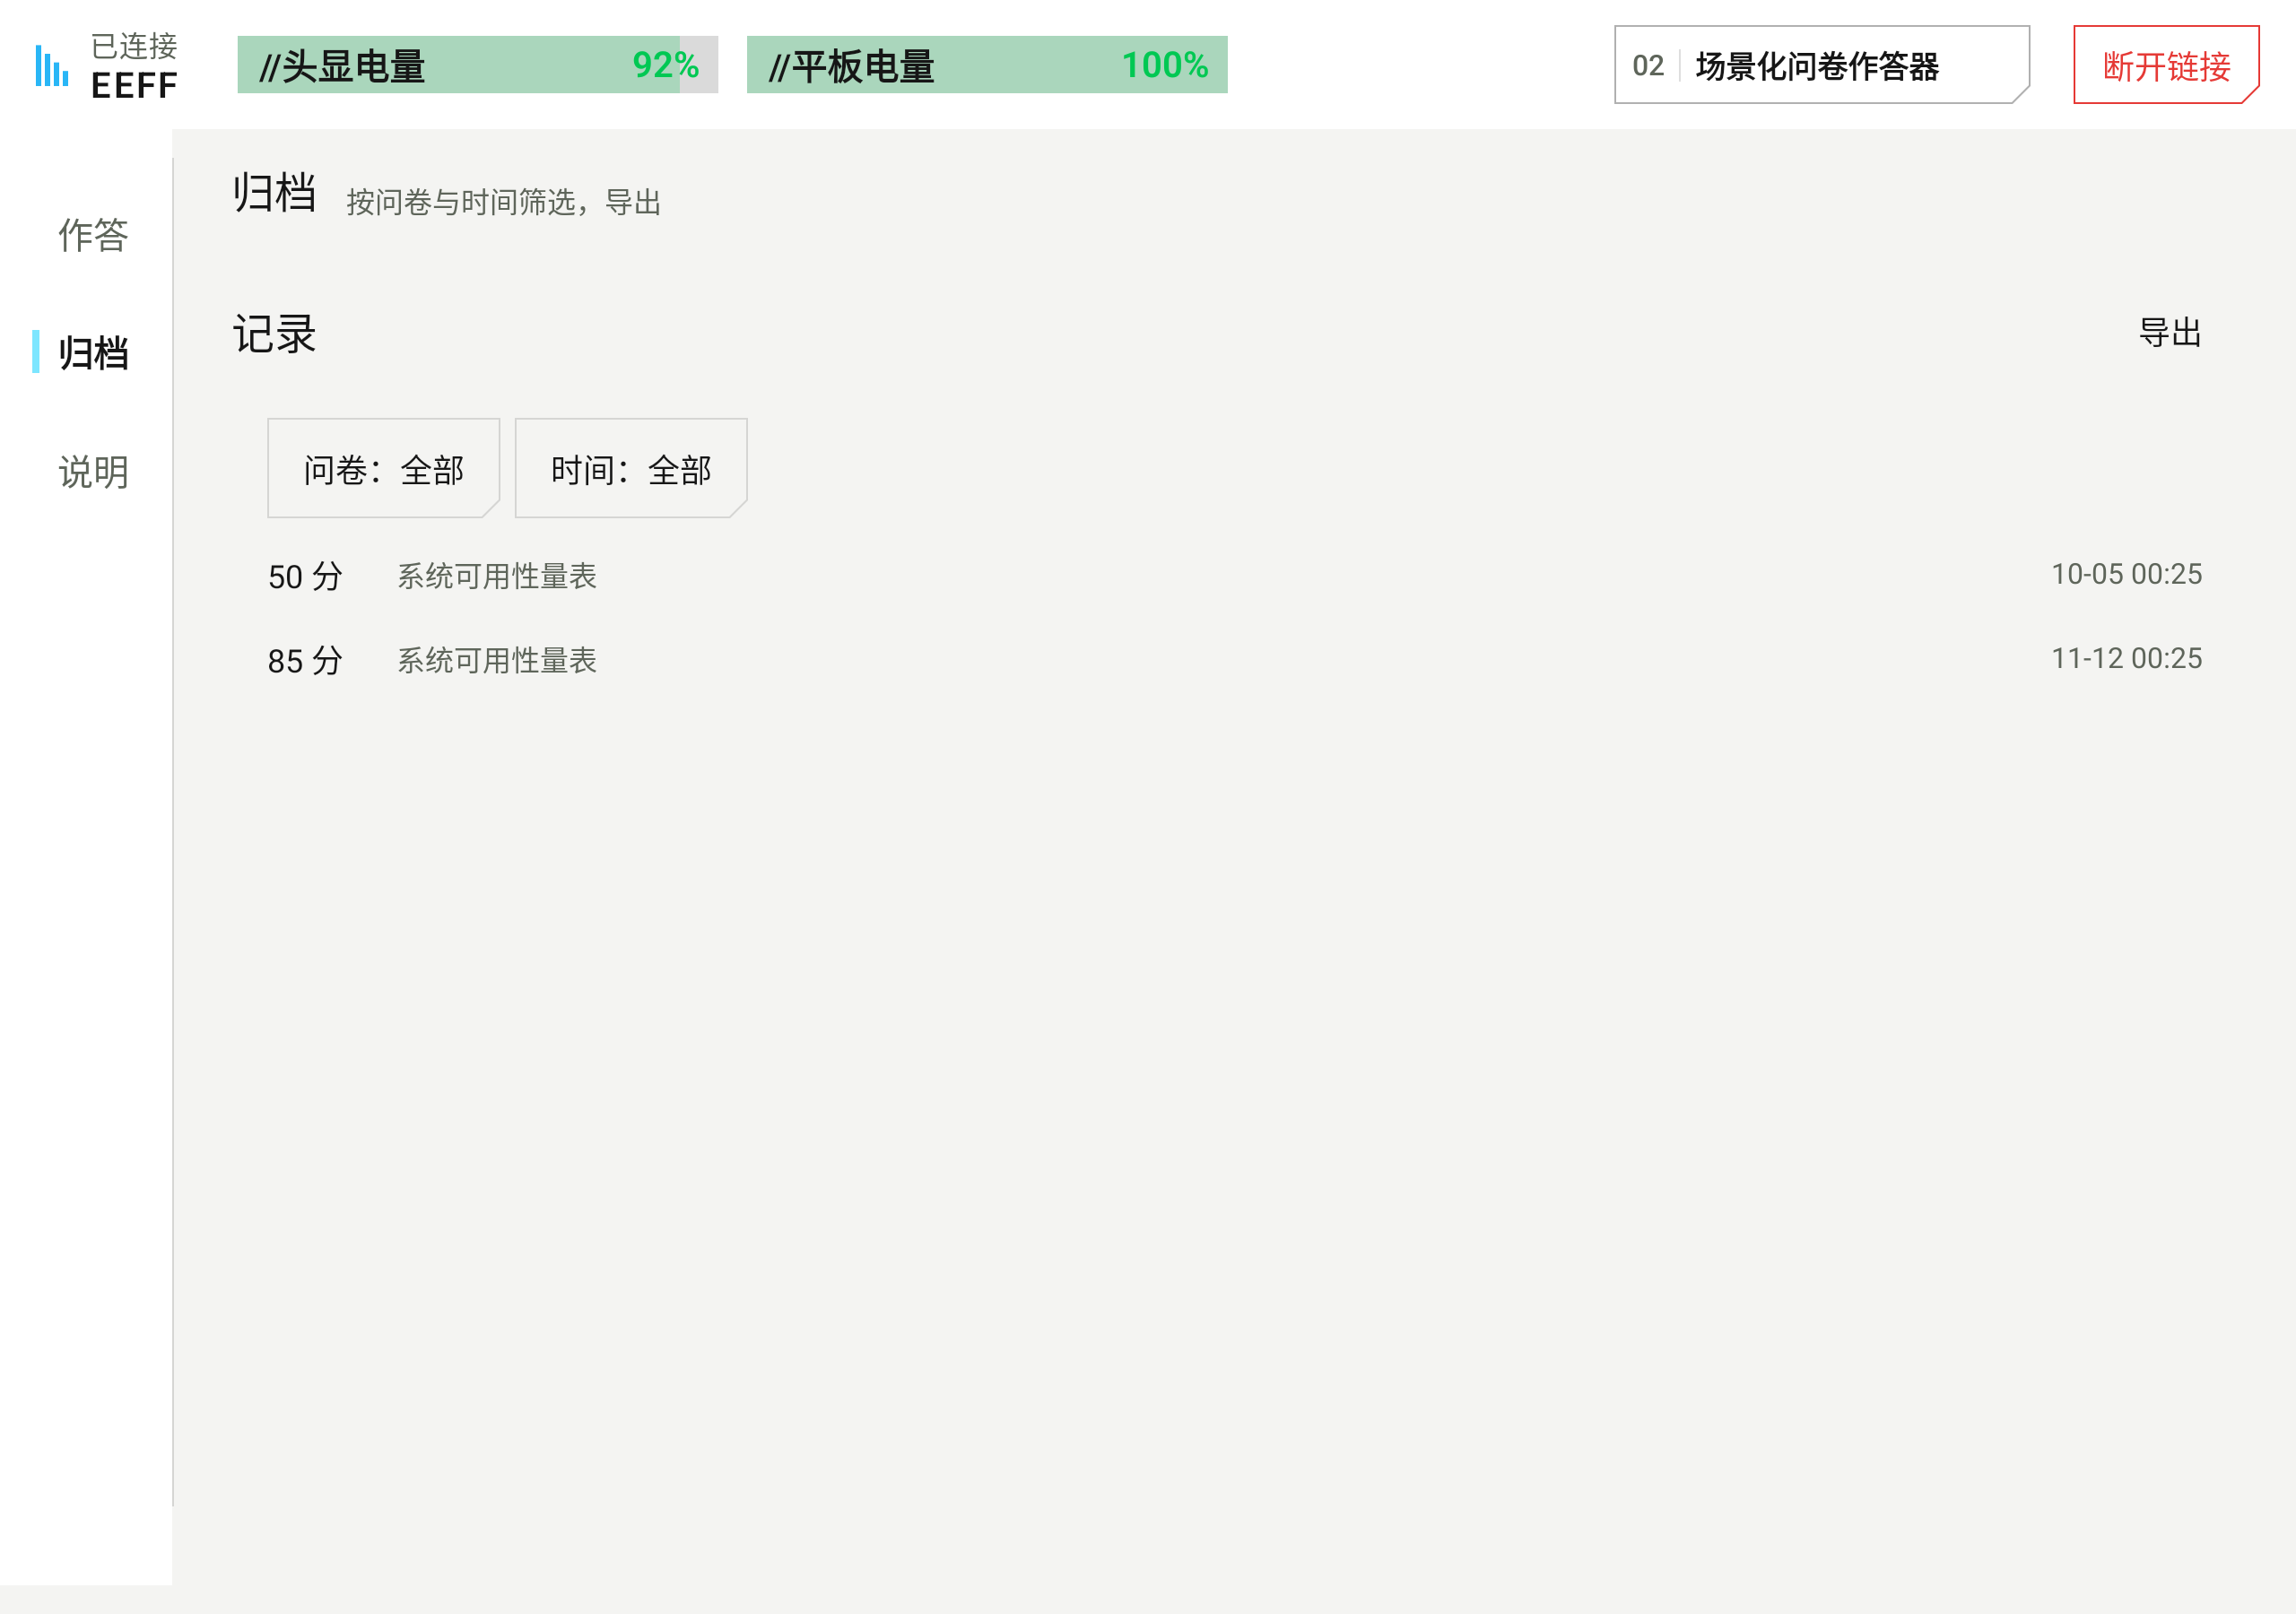
\includegraphics[keepaspectratio]{img/08-records.png}}

}

\caption{归档。可按问卷与时间筛选，再导出。}

\end{figure}%

\begin{itemize}
\tightlist
\item
  每份完成或部分完成的问卷按次归档，带完成时间与来源应用。
\item
  「问卷：全部」循环筛选量表；「时间：7 天」循环筛选时间窗。
\item
  「导出」走系统分享，生成 JSON；不自动上传。
\item
  记录只在本机。换平板或卸载应用前先导出。
\end{itemize}

\section{5 说明}\label{ux8bf4ux660e}

两个应用左栏的最后一项都是 \textbf{说明}，打开的是 \textbf{当前应用}
的说明书，显示在右侧主区域（不是弹窗，所以可以一边看一边操作）：

\begin{itemize}
\tightlist
\item
  场景化排尿引导器：连接、启动、标定、会话中的每一个控制块、故障处置。
\item
  场景化问卷作答器：施测、作答、归档与导出。
\end{itemize}

\begin{figure}[H]

{\centering \pandocbounded{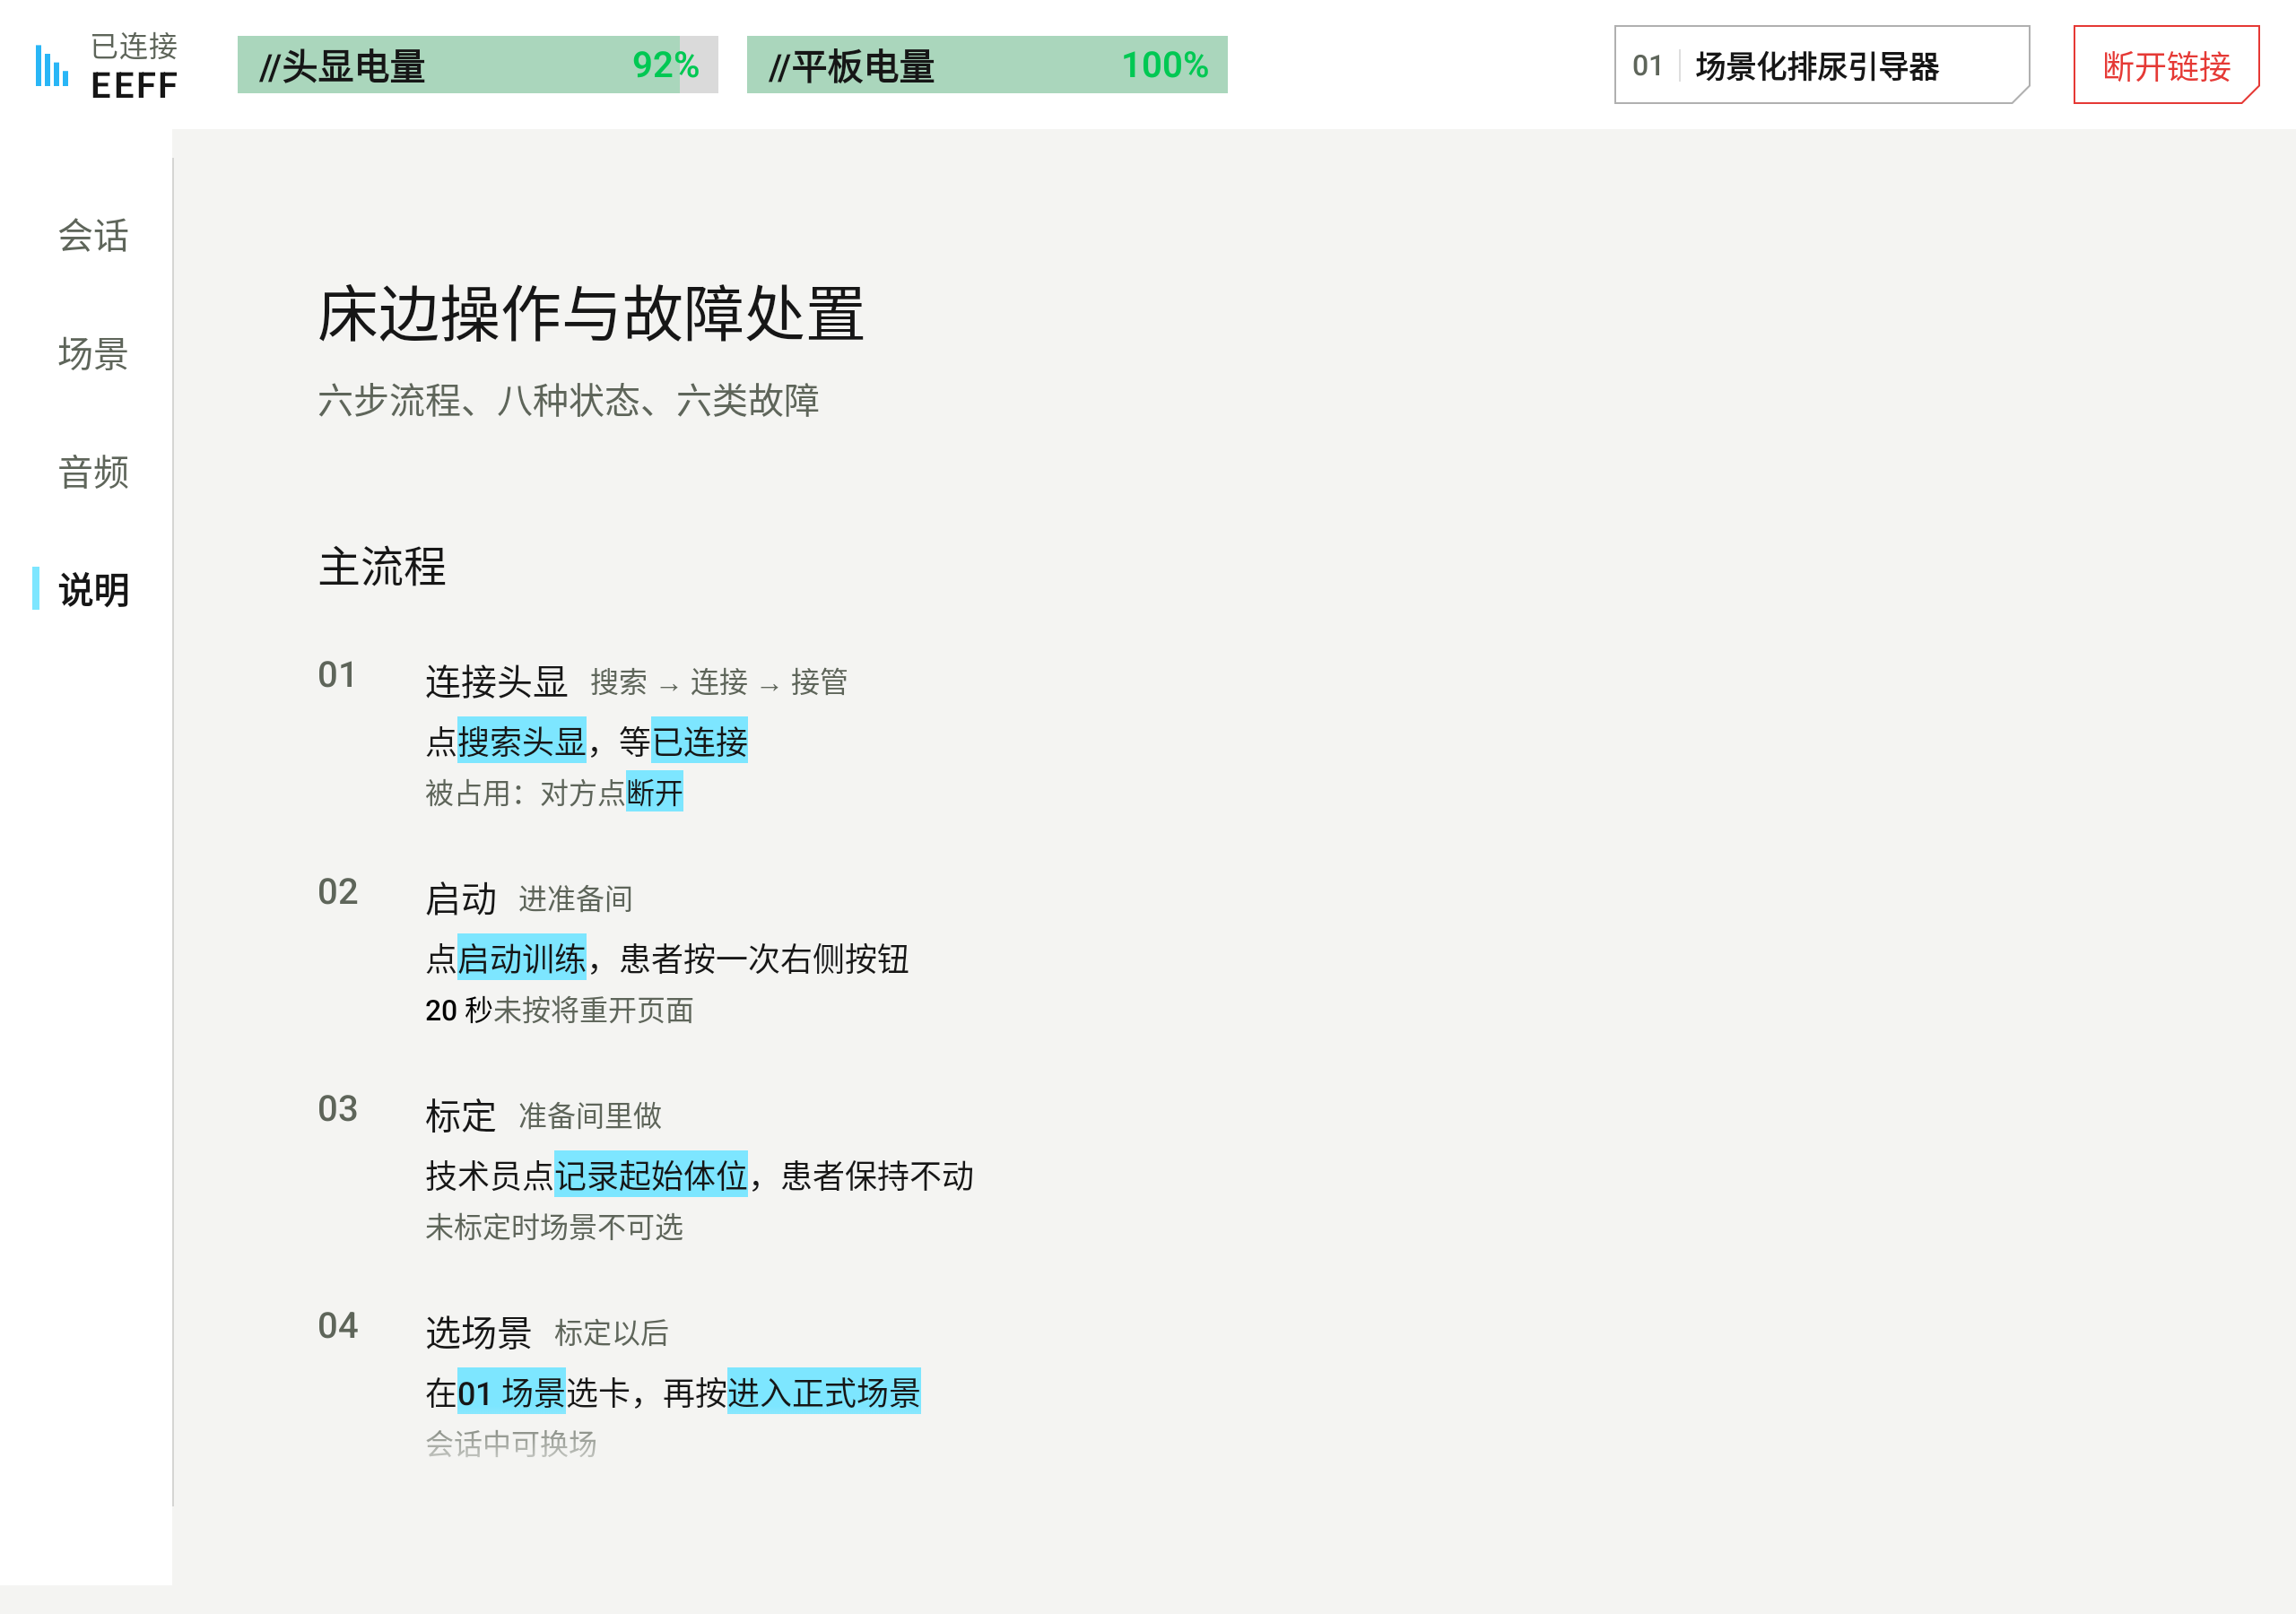
\includegraphics[keepaspectratio]{img/09-guide-training.png}}

}

\caption{场景化排尿引导器的说明页。}

\end{figure}%

\begin{figure}[H]

{\centering \pandocbounded{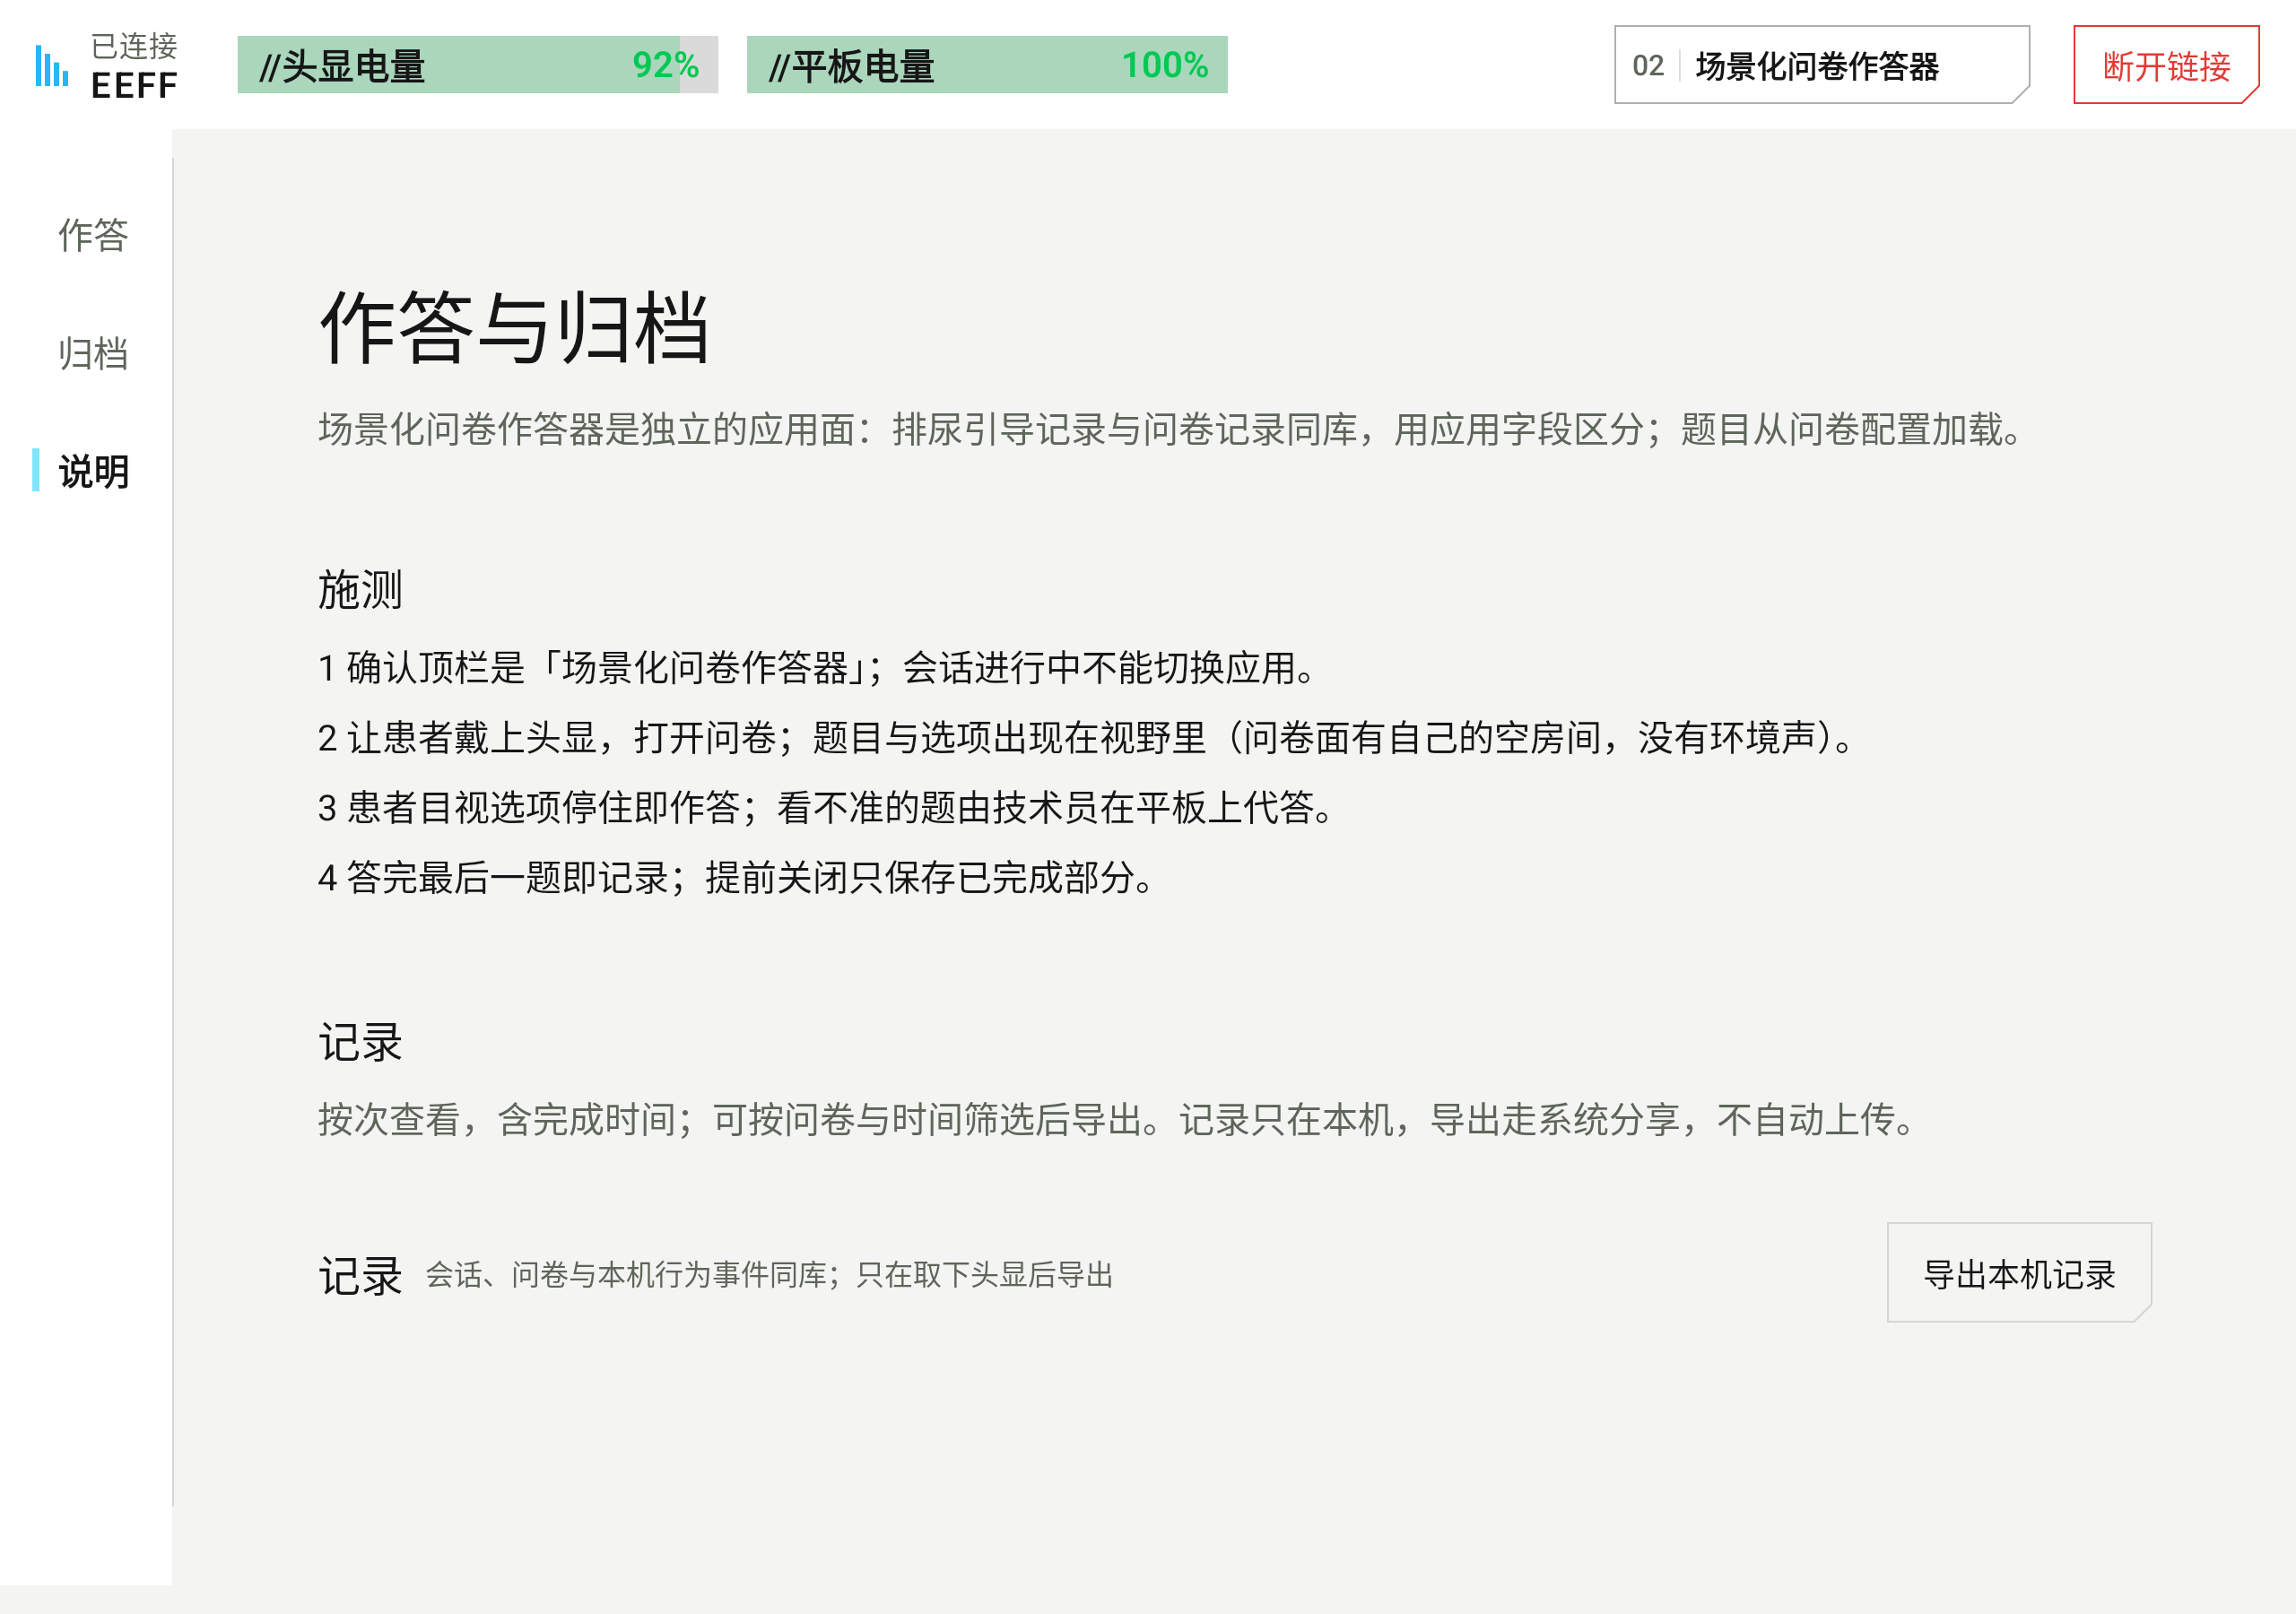
\includegraphics[keepaspectratio]{img/10-guide-questionnaire.png}}

}

\caption{场景化问卷作答器的说明页。}

\end{figure}%

首页左侧的三个标签只是摘要，不等同于说明。

\section{6
记录与会话台账}\label{ux8bb0ux5f55ux4e0eux4f1aux8bddux53f0ux8d26}

{\def\LTcaptype{none} % do not increment counter
\begin{longtable}[]{@{}
  >{\raggedright\arraybackslash}p{(\linewidth - 4\tabcolsep) * \real{0.3333}}
  >{\raggedright\arraybackslash}p{(\linewidth - 4\tabcolsep) * \real{0.3333}}
  >{\raggedright\arraybackslash}p{(\linewidth - 4\tabcolsep) * \real{0.3333}}@{}}
\toprule\noalign{}
\begin{minipage}[b]{\linewidth}\raggedright
记录
\end{minipage} & \begin{minipage}[b]{\linewidth}\raggedright
位置
\end{minipage} & \begin{minipage}[b]{\linewidth}\raggedright
内容
\end{minipage} \\
\midrule\noalign{}
\endhead
\bottomrule\noalign{}
\endlastfoot
会话摘要 & 本机 & 时长、场景、起伏、语音使用情况 \\
分段台账 & 本机 &
段序号、场景、实际秒数、峰值（换场与回准备间各成一段） \\
问卷记录 & 本机 & 题目答案、完成时间、来源应用、是否完整 \\
导出 & 场景化问卷作答器 → 归档 & JSON，经系统分享 \\
\end{longtable}
}

记录用于复盘与交接，不用于诊断。需要带走记录时，先导出，再清理平板。

\section{7 常见情况}\label{ux5e38ux89c1ux60c5ux51b5}

{\def\LTcaptype{none} % do not increment counter
\begin{longtable}[]{@{}ll@{}}
\toprule\noalign{}
现象 & 怎么做 \\
\midrule\noalign{}
\endhead
\bottomrule\noalign{}
\endlastfoot
搜不到头显 & 确认头显已开机、停在静岸入口；再点「搜索头显」 \\
一直连不上 & 看是否被另一台平板占用；让对方先「断开链接」 \\
页面没打开 & 点「启动训练」重新拉起页面，等 10 秒 \\
头显里一直黑屏 & 让患者保持不动；仍黑则重新「启动训练」 \\
患者说看不到场景 & 检查当前段与场景卡；必要时重新校准 \\
患者不适 & 立即点「结束」，再帮患者摘头显 \\
语音没声音 & 检查头显音量与耳机；点「下一句」重试 \\
想切换应用但按钮不可用 & 会话进行中；先「结束」，再切 \\
断开后头显没回来 & 等约 5 秒；仍未回则重新连接或重启头显应用 \\
问卷没有新记录 & 确认答完最后一题；检查归档筛选条件 \\
导出没有反应 & 系统分享没有可用目标；先在系统里登录/配置文件应用 \\
\end{longtable}
}

\section{8 安全与边界}\label{ux5b89ux5168ux4e0eux8fb9ux754c}

\begin{itemize}
\tightlist
\item
  患者不适、头晕、恶心：先「结束」，再摘头显。
\item
  患者在佩戴期间，技术员不离开床边。
\item
  本系统是体验性工具，不用于诊断或治疗。
\item
  场景切换当前是硬切；避免在语音中途切换，优先在段边界换场。
\item
  平板与头显只走本地蓝牙；问卷记录留在本机，导出由操作员发起。
\item
  头显电量低于 20\% 先充电；平板电量低时先接电源再开始。
\end{itemize}

\section{9 班前 / 班后检查}\label{ux73edux524d-ux73edux540eux68c0ux67e5}

\textbf{班前}

\begin{itemize}
\tightlist
\item[$\square$]
  头显与平板安装的是同一版本。
\item[$\square$]
  头显电量 ≥ 50\%，平板电量足够一次会话。
\item[$\square$]
  头显停在静岸入口，蓝牙可见。
\item[$\square$]
  平板能搜到头显并连接。
\item[$\square$]
  试一句语音，确认耳机有声。
\item[$\square$]
  让患者按一次头显按钮，确认入口正常。
\item[$\square$]
  与患者说明：随时可以说停。
\end{itemize}

\textbf{班后}

\begin{itemize}
\tightlist
\item[$\square$]
  会话已「结束」，患者已摘头显。
\item[$\square$]
  需要时完成问卷。
\item[$\square$]
  导出本次记录。
\item[$\square$]
  「断开链接」，头显放回充电位。
\end{itemize}

\section{10 版本与验证}\label{ux7248ux672cux4e0eux9a8cux8bc1}

\textbf{v2.1 的主要变化}

\begin{itemize}
\tightlist
\item
  体位：一条 0--100\% 的补偿滑条（按即接管、限速跟随、松手保持）+
  整数秒的时长填空 + 修正 / 逆修正 /
  暂停三个键。起身与躺下共用同一个时长。
\item
  起伏：0--3 级改成 0--100\%，并多一个「呼吸」开关；场景可以把上限声明为
  0（准备间即如此），这时整块控制不可用并写明原因。
\item
  会话页左列：标题卡、画面（三分之二）、读数卡（含双水平盘）、水声卡；右列：场景
  / 起伏 / 体位 / 结束会话。
\item
  读数卡的小盘同时画真实水平与虚拟水平，给出还没补偿完的角度。
\item
  场景块常驻「切换场景」，选中项与实机一致时置灰；页头「准备间」可以把人送回中性空房，会话不结束、校准保留。
\item
  换场过四分之一秒黑幕，不再硬切。
\item
  导航：左栏单行中文，当前项用冰蓝游标；两个应用的最后一项都是
  \textbf{说明}，说明书显示在右侧主区域。
\item
  顶栏：电量改为并排的两个短字段；说明书按钮移出顶栏；\texttt{结束会话}
  与 \texttt{断开链接} 分开命名与着墨。
\item
  手动重新校准跳过稳定等待；取样期头部偏转超过 12°
  会从当前姿态重开窗口。
\end{itemize}

\textbf{验证范围}

\begin{itemize}
\tightlist
\item
  平板界面截图来自 2560 × 1800 模拟器；本册中的图按此比例。
\item
  TypeScript 测试与 Kotlin 协议/控制端单测通过。
\item
  真机 BLE、头显 WebXR 与现场手感需在设备上按第 9
  节复验；本机没有真实头显可连。
\end{itemize}




\end{document}
